\documentclass[10pt,a4paper]{article}

\usepackage[T1]{fontenc}
\usepackage[utf8]{inputenc}
\usepackage[margin=0.72in, top=0.7in, bottom=0.72in]{geometry}
\usepackage{amsmath,amssymb}
\usepackage{array}
\usepackage{booktabs}
\usepackage{graphicx}
\usepackage{xcolor}
\usepackage{framed}
\usepackage{enumitem}
\usepackage{float}
\usepackage{fancyvrb}
\usepackage{titlesec}
\usepackage[colorlinks=true,linkcolor=NavyBlue,urlcolor=NavyBlue,citecolor=NavyBlue]{hyperref}

\definecolor{NavyBlue}{RGB}{22,68,128}
\definecolor{SoftBg}{RGB}{244,247,250}
\definecolor{RuleGray}{RGB}{205,213,222}
\definecolor{CodeBg}{RGB}{247,248,250}

\titleformat{\section}{\large\bfseries\color{NavyBlue}}{\thesection.}{0.55em}{}[\vspace{-0.4em}\color{RuleGray}\rule{\textwidth}{0.6pt}]
\titleformat{\subsection}{\normalsize\bfseries\color{NavyBlue!85!black}}{\thesubsection}{0.5em}{}
\titlespacing*{\section}{0pt}{1.1em}{0.45em}
\titlespacing*{\subsection}{0pt}{0.7em}{0.3em}

\setlength{\parindent}{0pt}
\setlength{\parskip}{0.42em}
\setlist{nosep, leftmargin=1.4em}

% Simple callout box using framed (available in TinyTeX)
\newenvironment{notebox}[1][Key Idea]{%
  \def\FrameCommand{\fboxsep=6pt\fcolorbox{NavyBlue!45!white}{SoftBg}}%
  \MakeFramed{\advance\hsize-\width\FrameRestore}%
  \noindent\textbf{\color{NavyBlue}#1:} \ignorespaces
}{\endMakeFramed}

\begin{document}

% --- Header / Title Banner ---
\begin{center}
  {\LARGE\bfseries\color{NavyBlue} Understanding PID Control from Scratch}\\[0.35em]
  {\normalsize\color{black!75} Intuition, Mathematics, Python Simulations, and Real-World Engineering Fixes}
\end{center}
\vspace{-0.3em}
\noindent\color{RuleGray}\rule{\textwidth}{0.8pt}\color{black}

\begin{notebox}[What This Guide Covers]
PID (Proportional--Integral--Derivative) control is the workhorse algorithm behind cruise control, drones, robot arms, 3D printers, and industrial motors. This guide teaches PID from zero prior background: every topic begins with a plain-English idea, backs it up with exact formulas, and proves it with reproducible Python (NumPy + Matplotlib) graphs.
\end{notebox}

% ============================================================================
\section{The Basic Idea}
% ============================================================================
Imagine adjusting a shower to a comfortable \textbf{38\,$^\circ$C} when the water starts freezing cold at 15\,$^\circ$C. You do not calculate pipe fluid dynamics in your head. Instead, you repeat a simple three-step loop:
\begin{enumerate}
  \item \textbf{Measure:} Feel the water temperature with your hand (\textit{sensor}).
  \item \textbf{Compare:} Notice how far the actual temperature is from your 38\,$^\circ$C goal (\textit{error} $= 38 - 15 = +23\,^\circ\text{C}$).
  \item \textbf{Act:} Turn the hot valve (\textit{controller}) by a lot when it is far off, a little when it is close, and back off if it warms up too fast.
\end{enumerate}

In engineering, the machine being controlled (pipes, motor, car, or spring-mass) is called the \textbf{plant}. The desired goal is the \textbf{setpoint} $r(t)$, the measured output is $y(t)$, and the gap $e(t) = r(t) - y(t)$ is the \textbf{error}. Because the sensor feeds the output back to the input to compute the error, this is called a \textbf{closed-loop feedback system} (Figure~\ref{fig:loop}).

\begin{figure}[H]
  \centering
  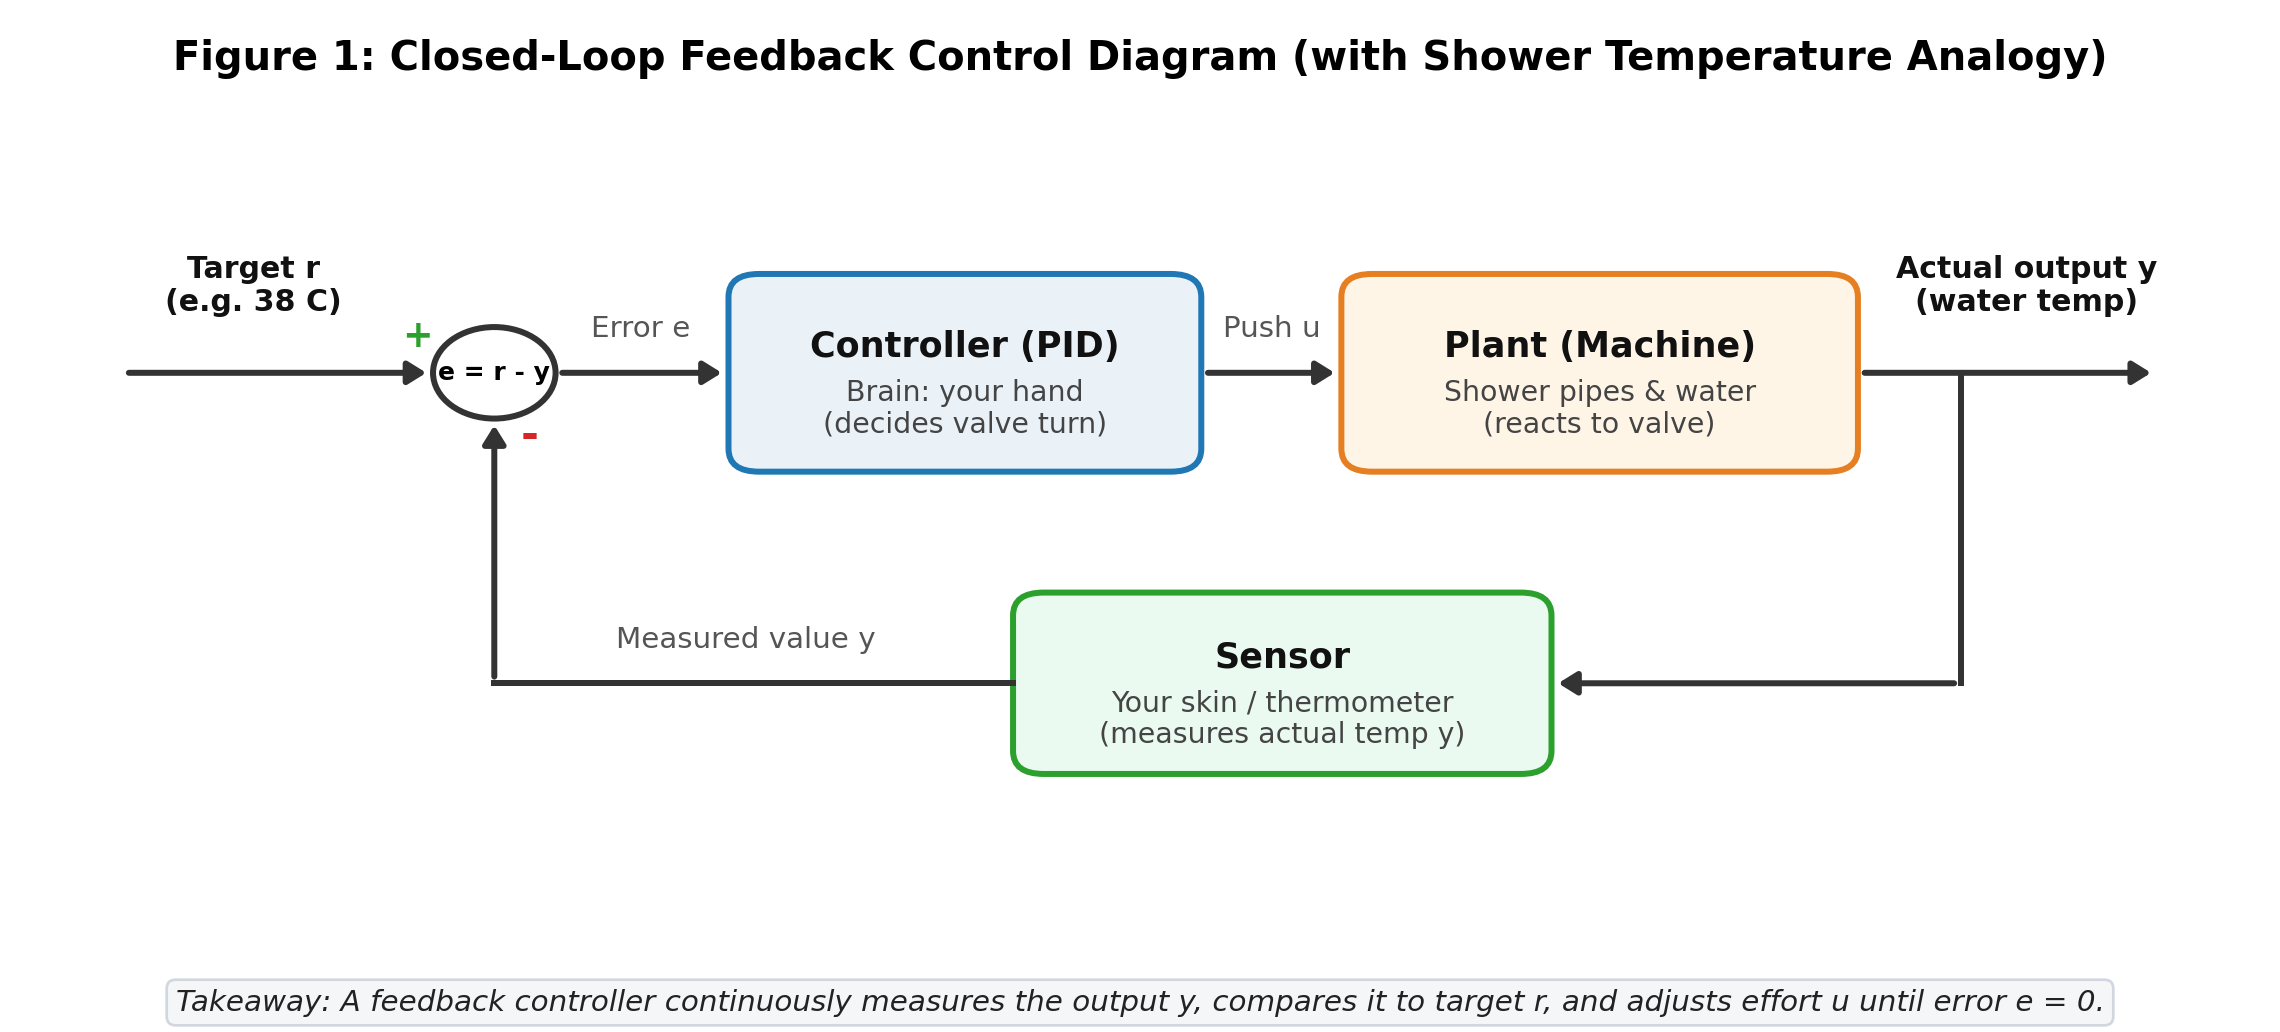
\includegraphics[width=0.94\textwidth]{figures/fig01_feedback_loop.png}
  \caption{Closed-loop feedback structure: the controller continuously shrinks the gap $e = r - y$ using live sensor feedback.}
  \label{fig:loop}
\end{figure}

% ============================================================================
\section{The PID Formula}
% ============================================================================
A PID controller turns the error $e(t) = r(t) - y(t)$ into a control command $u(t)$ by adding three simple reactions---to the \textbf{present}, the \textbf{past}, and the \textbf{trend (future)} of the error:
\begin{equation}
  u(t) = \underbrace{K_p\, e(t)}_{\text{P: present error}}
       + \underbrace{K_i \int_0^t e(\tau)\,d\tau}_{\text{I: accumulated past error}}
       + \underbrace{K_d\, \frac{de(t)}{dt}}_{\text{D: rate of change}}
  \label{eq:pid_cont}
\end{equation}

\textbf{What each letter means and its units} (illustrated for our position test system, where position $y$ is in meters $\text{m}$, time $t$ is in seconds $\text{s}$, and motor push $u$ is in Newtons $\text{N}$; for other plants, units scale with output and actuator units):
\begin{itemize}
  \item $r(t)$ ($\text{m}$): \textbf{Setpoint} (target position). \quad $y(t)$ ($\text{m}$): \textbf{Measured output} (actual position).
  \item $e(t) = r(t) - y(t)$ ($\text{m}$): \textbf{Error} (positive means we are short of the target; negative means we overshot).
  \item $u(t)$ ($\text{N}$): \textbf{Control effort} sent to the actuator/motor.
  \item $K_p$ ($\text{N/m}$): \textbf{Proportional gain}. Pushes harder the larger the \emph{present} error is (like a virtual spring pulling toward the target).
  \item $K_i$ ($\text{N}/(\text{m}\cdot\text{s})$): \textbf{Integral gain}. Adds up all \emph{past} error over time; even a tiny lingering gap eventually builds enough push to erase steady-state error.
  \item $K_d$ ($\text{N}\cdot\text{s/m}$): \textbf{Derivative gain}. Reacts to \emph{how fast the error is changing}; as the machine races toward the target, $\frac{de}{dt}$ is negative, so D applies a braking force to prevent overshoot.
\end{itemize}

\textbf{How a computer runs PID step by step:} A microcontroller wakes up every small time step $\Delta t$ (for example, $\Delta t = 0.005\text{ s}$ at $200\text{ Hz}$). Replacing the integral with a running sum and the derivative with a slope between consecutive samples gives the discrete algorithm at step $k$:
\begin{equation}
  e_k = r_k - y_k, \qquad
  I_k = I_{k-1} + e_k\,\Delta t, \qquad
  D_k = \frac{e_k - e_{k-1}}{\Delta t}, \qquad
  u_k = K_p e_k + K_i I_k + K_d D_k.
  \label{eq:pid_disc}
\end{equation}

% ============================================================================
\section{The Test System (Given)}
% ============================================================================
To test every PID concept with real numbers, we simulate a \textbf{1\,kg block on a spring with a damper} (just like one corner of a car suspension): mass $m = 1\text{ kg}$, viscous damping $c = 10\text{ N}\cdot\text{s/m}$, and spring stiffness $k = 20\text{ N/m}$. Starting at rest ($x(0)=0\text{ m}$, $\dot{x}(0)=0\text{ m/s}$), the goal is to move and hold the block at $r = 1.0\text{ m}$.

By Newton's second law ($m\ddot{x} = \sum F$), the motor force $u(t)$ pushes forward while the damper resists motion ($-c\dot{x}$) and the spring pulls back ($-kx$):
\begin{equation}
  m\ddot{x}(t) + c\dot{x}(t) + kx(t) = u(t)
  \quad\Longrightarrow\quad
  \ddot{x}(t) + 10\dot{x}(t) + 20x(t) = u(t).
  \label{eq:plant}
\end{equation}
For numerical integration (4th-order Runge--Kutta in \texttt{systems.py}), we rewrite Eq.~\eqref{eq:plant} as two first-order equations for position $x$ and velocity $v = \dot{x}$:
\[
  \dot{x} = v, \qquad \dot{v} = \frac{u - 10v - 20x}{1}.
\]

\textbf{Why the spring needs a constant push to stay at $1\text{ m}$:} Once the block reaches $x = 1.0\text{ m}$ and stops moving ($\dot{x}=0$, $\ddot{x}=0$), the damper force vanishes ($10\times 0 = 0$), but the stretched spring pulls backward with $k x = 20 \times 1.0 = 20\text{ N}$. Setting $\dot{x}=\ddot{x}=0$ in Eq.~\eqref{eq:plant} shows that \textbf{the motor must keep pushing with a constant $u_{\infty} = 20\text{ N}$ forever}, otherwise the spring yanks the block back toward $0\text{ m}$. Figure~\ref{fig:testsys} confirms this open-loop test: $20\text{ N}$ holds at $1.00\text{ m}$, whereas $10\text{ N}$ stops halfway at $0.50\text{ m}$.

\begin{figure}[H]
  \centering
  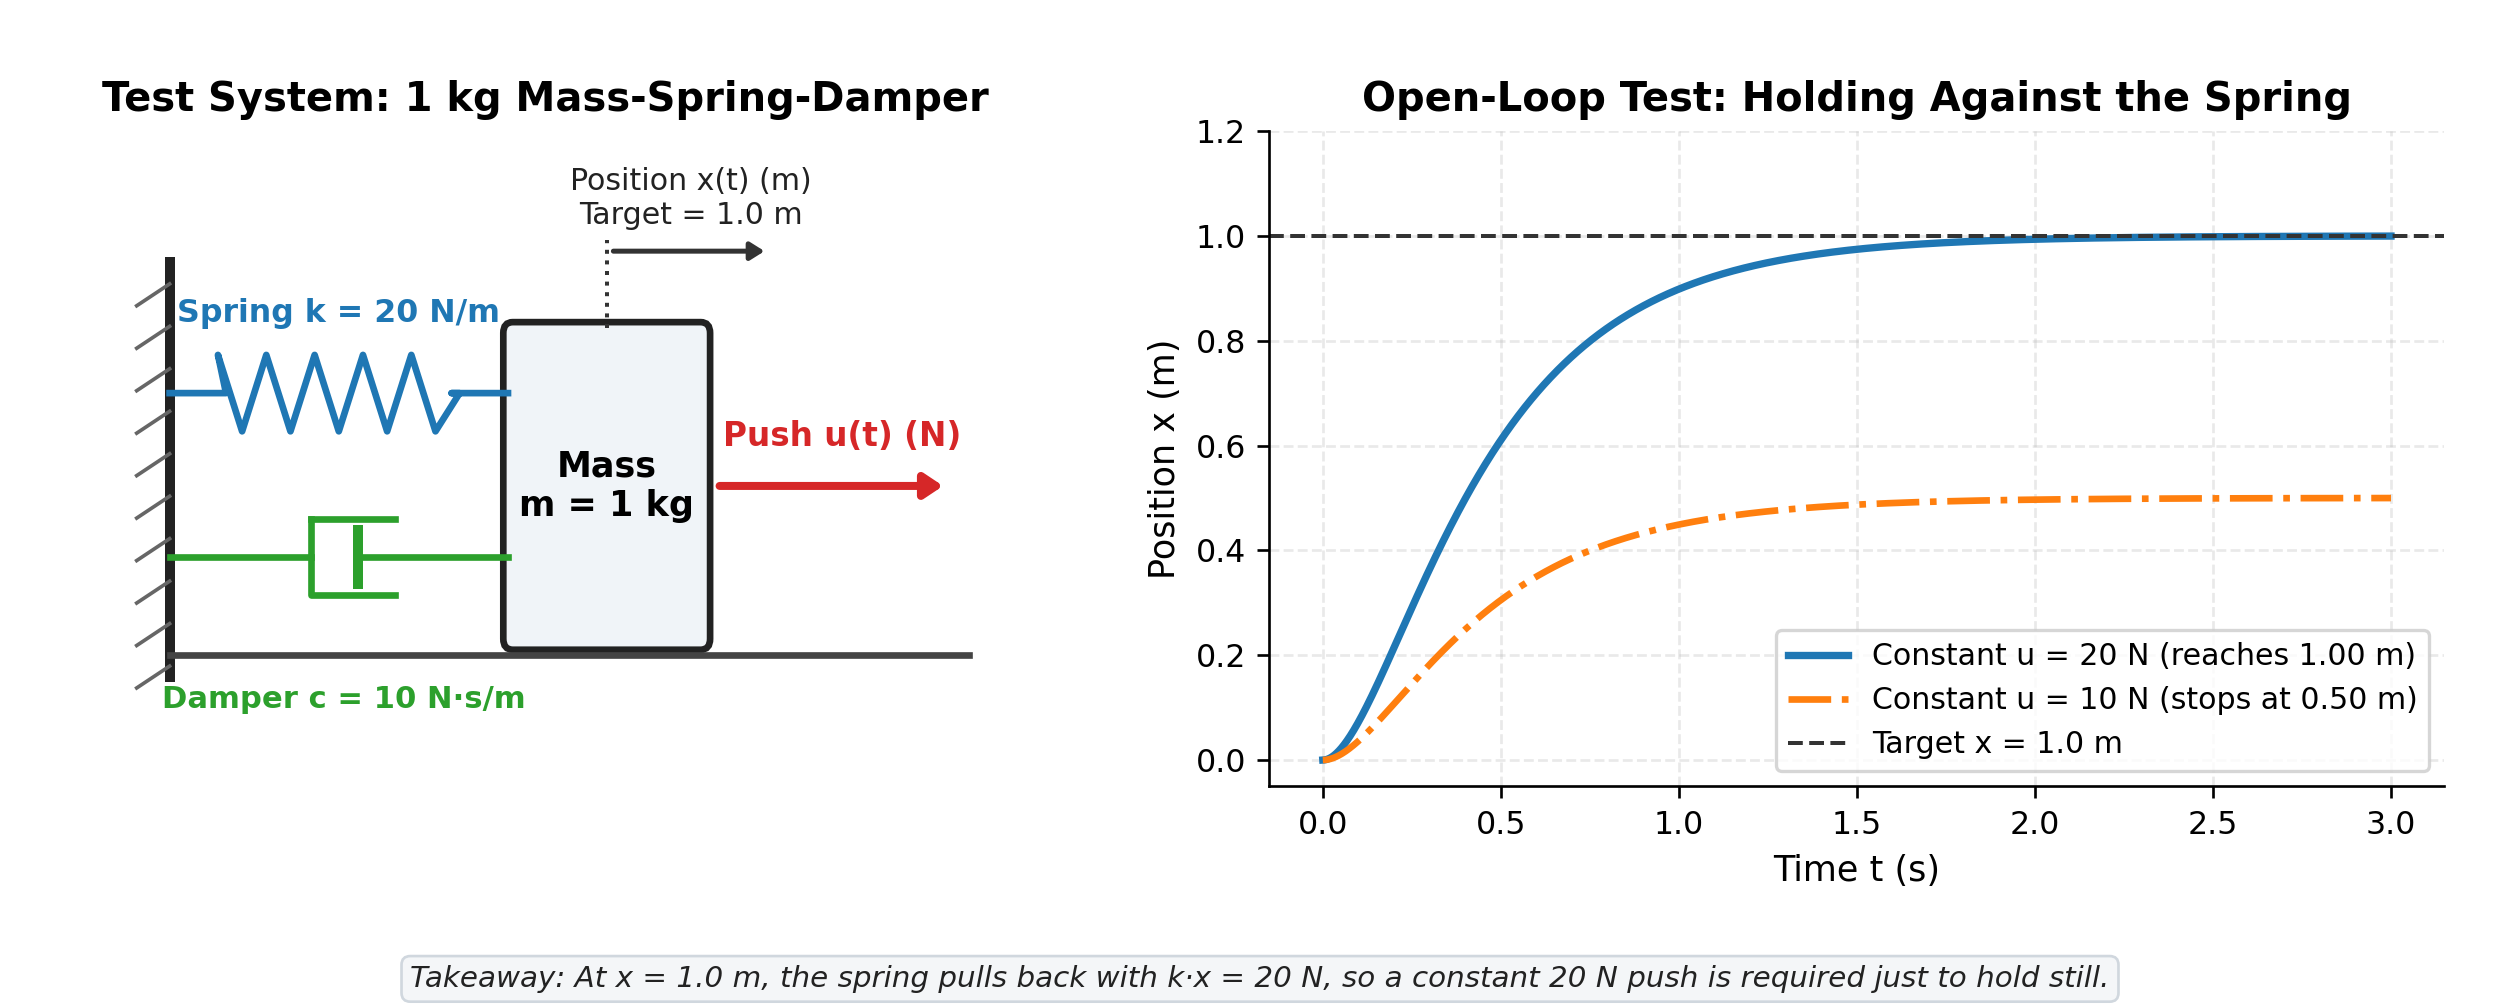
\includegraphics[width=0.98\textwidth]{figures/fig02_test_system.png}
  \caption{Left: 1\,kg mass-spring-damper test plant. Right: open-loop step tests proving $u = 20\text{ N}$ is required to hold $x = 1.00\text{ m}$.}
  \label{fig:testsys}
\end{figure}

% ============================================================================
\section{How to Judge a Result}
% ============================================================================
Before tuning gains, we need four clear numbers to judge any step response (moving from $0\text{ m}$ toward target $r = 1.0\text{ m}$):
\begin{enumerate}
  \item \textbf{Rise time ($t_r$, $\text{s}$):} How fast it rises---the time from reaching $10\%$ of its final steady value $y_{\text{ss}}$ to reaching $90\%$ of $y_{\text{ss}}$.
  \item \textbf{Overshoot ($\%\text{OS}$, $\%$):} How far past $y_{\text{ss}}$ it swings before turning back: $\%\text{OS} = \max\!\left(0,\,\frac{x_{\text{peak}} - y_{\text{ss}}}{y_{\text{ss}}}\right)\times 100\%$.
  \item \textbf{Settling time ($t_s$, $\text{s}$):} How long until bouncing dies out and $x(t)$ stays inside the $\pm 2\%$ band around $y_{\text{ss}}$ forever.
  \item \textbf{Steady-state error ($e_{\text{ss}}$, $\text{m}$):} How far from the target $r$ it finally stops: $e_{\text{ss}} = |r - y_{\text{ss}}|$.
\end{enumerate}

Figure~\ref{fig:metrics} marks all four measures on a single step response of our test system using P-only control ($K_p = 180$): it rises fast ($t_r = 0.098\text{ s}$), overshoots by $30.9\%$ (peaking at $1.178\text{ m}$), settles in $t_s = 0.777\text{ s}$, and stops short at $y_{\text{ss}} = 0.90\text{ m}$ ($e_{\text{ss}} = 0.10\text{ m}$).

\begin{figure}[H]
  \centering
  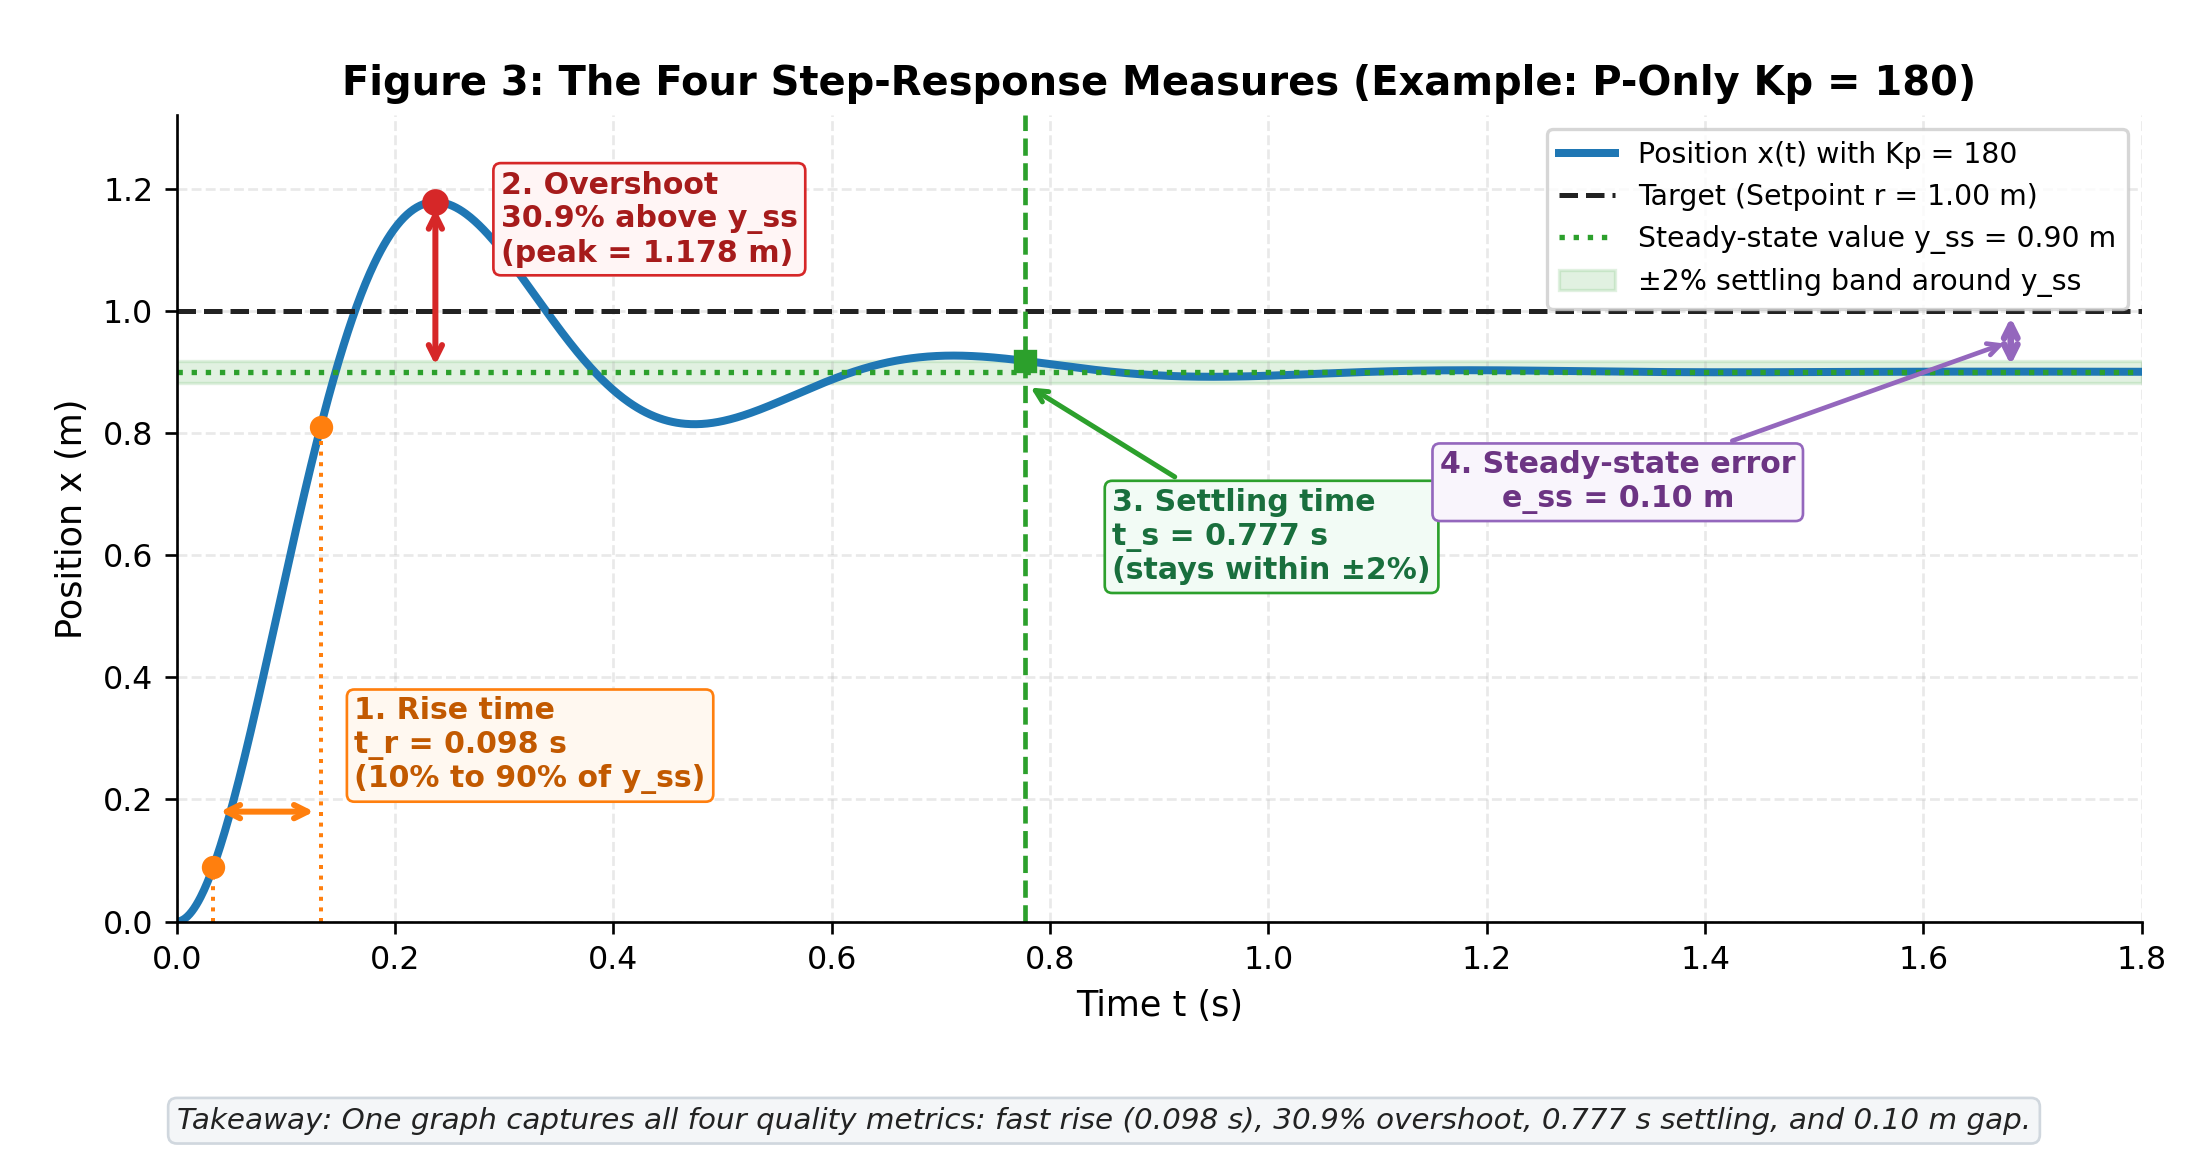
\includegraphics[width=0.92\textwidth]{figures/fig03_step_metrics.png}
  \caption{All four step-response measures annotated on a single response ($K_p = 180$).}
  \label{fig:metrics}
\end{figure}

% ============================================================================
\section{Each Part Alone (With Analytical Proofs)}
% ============================================================================

\subsection{Proportional Only (P): Fast, Simple, Always Stops Short}
With $K_i = K_d = 0$, the controller applies $u(t) = K_p(r - x)$. Plugging this into Eq.~\eqref{eq:plant} gives:
\begin{equation}
  \ddot{x} + 10\dot{x} + (20 + K_p)x = K_p r.
  \label{eq:p_closed}
\end{equation}
\textbf{Exact steady-state calculation:} At steady state, motion stops ($\dot{x} = \ddot{x} = 0$), so $(20 + K_p)x_{\text{ss}} = K_p r$:
\begin{equation}
  x_{\text{ss}} = \frac{K_p}{K_p + k}\,r = \frac{K_p}{K_p + 20}\text{ m}, \qquad
  e_{\text{ss}} = r - x_{\text{ss}} = \frac{20}{K_p + 20}\text{ m}.
  \label{eq:p_ss}
\end{equation}
Why can P alone \emph{never} reach $1.0\text{ m}$? Because at $x = 1.0\text{ m}$ the error is $e = 0$, so a P-only controller pushes with $u = K_p \cdot 0 = 0\text{ N}$---yet Section~3 proved the spring needs $20\text{ N}$! So the block must settle below $1\text{ m}$ where $K_p e_{\text{ss}} = 20\,x_{\text{ss}}$. Table~\ref{tab:p_only} and Figure~\ref{fig:p_only} show exact agreement between Eq.~\eqref{eq:p_ss} and our simulation across four strengths ($K_p \in \{10, 40, 100, 200\}$): raising $K_p$ shrinks $e_{\text{ss}}$ from $0.667\text{ m}$ to $0.091\text{ m}$ and speeds up rise time ($0.537\text{ s} \to 0.092\text{ s}$), but triggers $32.9\%$ overshoot at $K_p = 200$.

\begin{table}[H]
  \centering
  \small
  \begin{tabular}{ccccccc}
    \toprule
    $K_p$ ($\text{N/m}$) & Formula $x_{\text{ss}}$ ($\text{m}$) & Simulated $x_{\text{ss}}$ ($\text{m}$) & $e_{\text{ss}}$ ($\text{m}$) & Rise time $t_r$ ($\text{s}$) & Overshoot ($\%$) & Settling $t_s$ ($\text{s}$) \\
    \midrule
    10  & 0.3333 & 0.3333 & 0.6667 & 0.537 & 0.09  & 0.883 \\
    40  & 0.6667 & 0.6667 & 0.3333 & 0.254 & 7.09  & 0.776 \\
    100 & 0.8333 & 0.8333 & 0.1667 & 0.142 & 20.16 & 0.761 \\
    200 & 0.9091 & 0.9091 & 0.0909 & 0.092 & 32.88 & 0.749 \\
    \bottomrule
  \end{tabular}
  \caption{P-only analytical vs.\ simulated results: steady-state predictions match simulation to four decimal places.}
  \label{tab:p_only}
\end{table}

\begin{figure}[H]
  \centering
  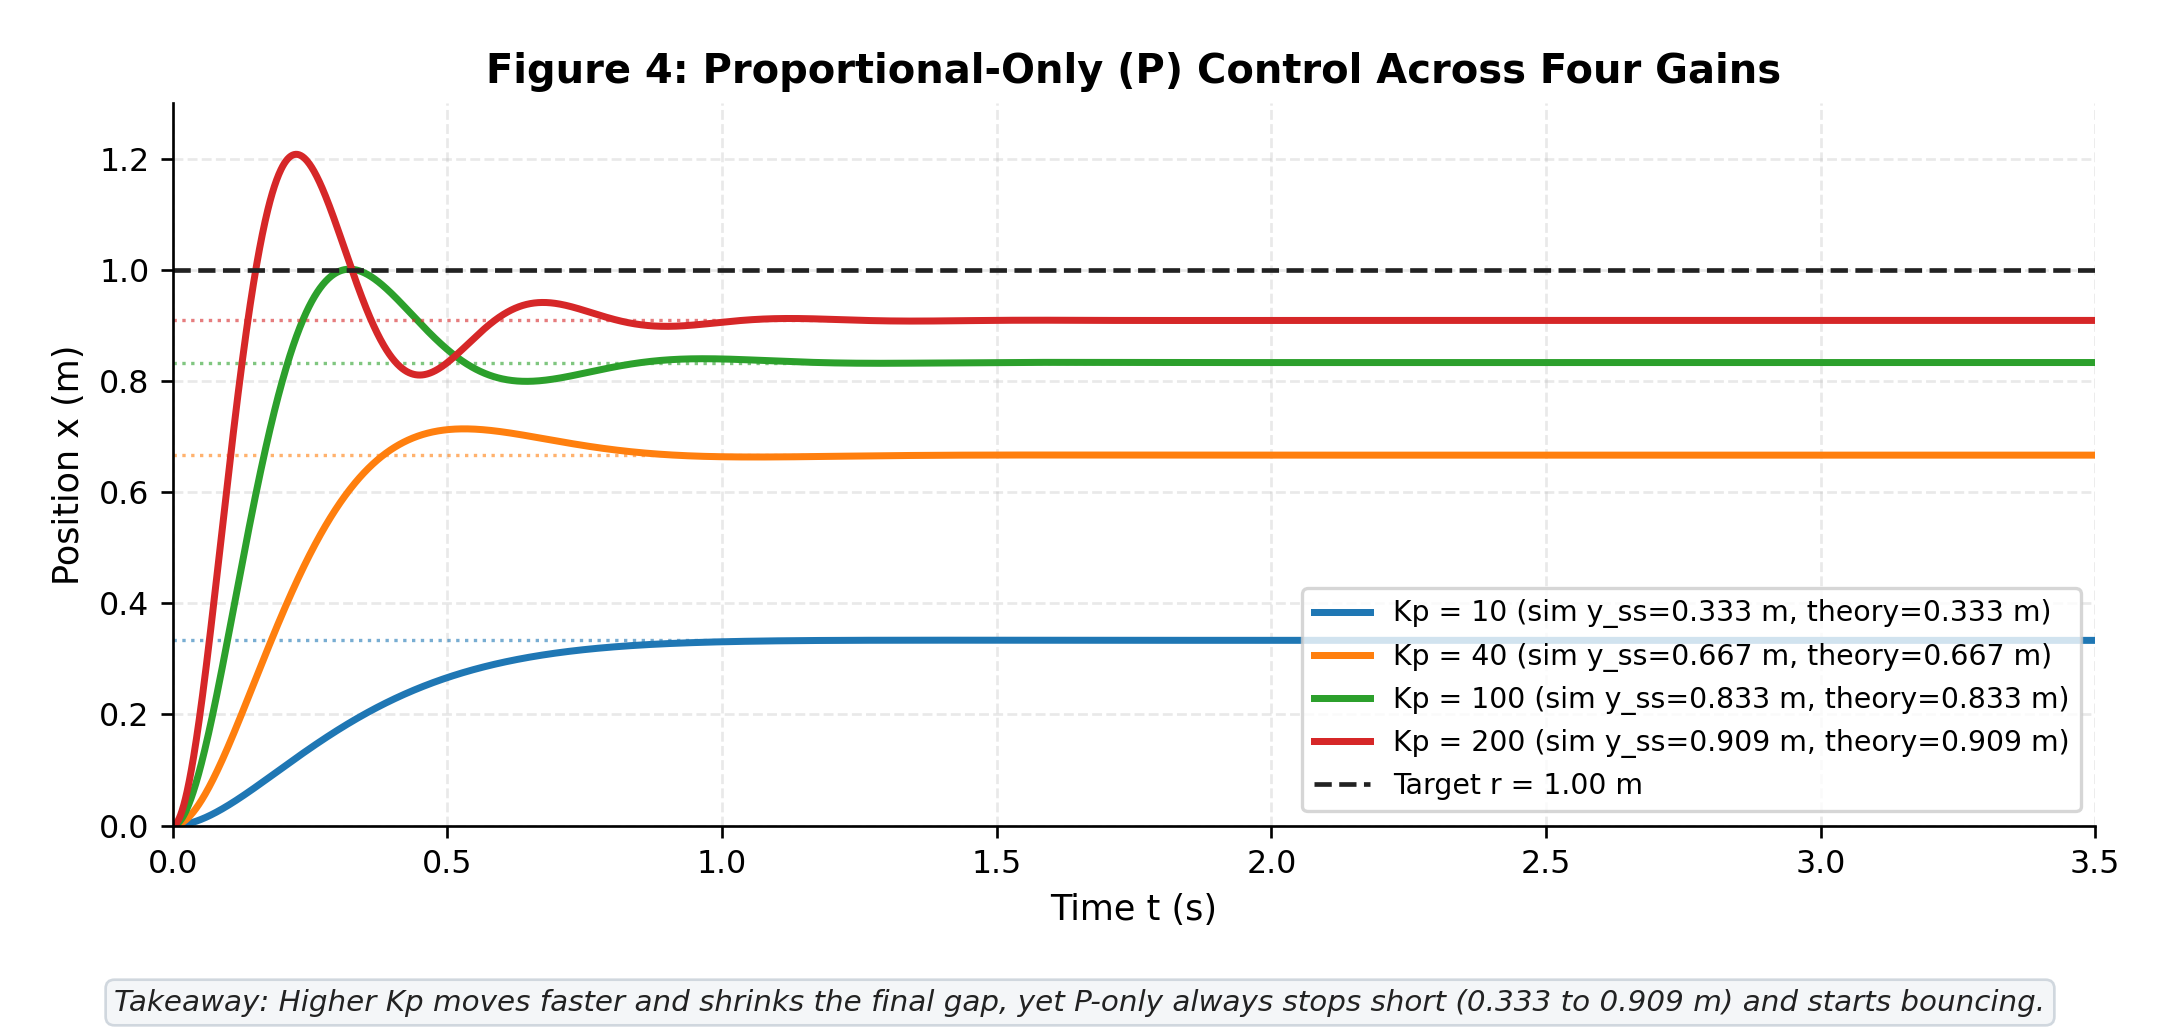
\includegraphics[width=0.90\textwidth]{figures/fig04_p_only.png}
  \caption{P-only responses for $K_p \in \{10, 40, 100, 200\}$ with theoretical steady-state dotted lines.}
  \label{fig:p_only}
\end{figure}

\subsection{Adding Integral (PI): Erasing the Final Gap}
To supply the constant $20\text{ N}$ holding force even when $e = 0$, we add the I term ($K_p = 60$, varying $K_i \in \{0, 60, 150, 350\}$). As long as $x < 1\text{ m}$, the running integral $\int e\,dt$ keeps growing, pushing the block up until $e = 0$ and the stored integral holds $K_i \int_0^\infty e(\tau)\,d\tau = 20\text{ N}$. As Figure~\ref{fig:pi} shows, adding $K_i = 150$ removes the entire $0.250\text{ m}$ steady-state gap ($e_{\text{ss}} = 0.0000\text{ m}$), though pushing $K_i = 350$ makes the controller wind up too much force early on and overshoot by $46.8\%$.

\begin{figure}[H]
  \centering
  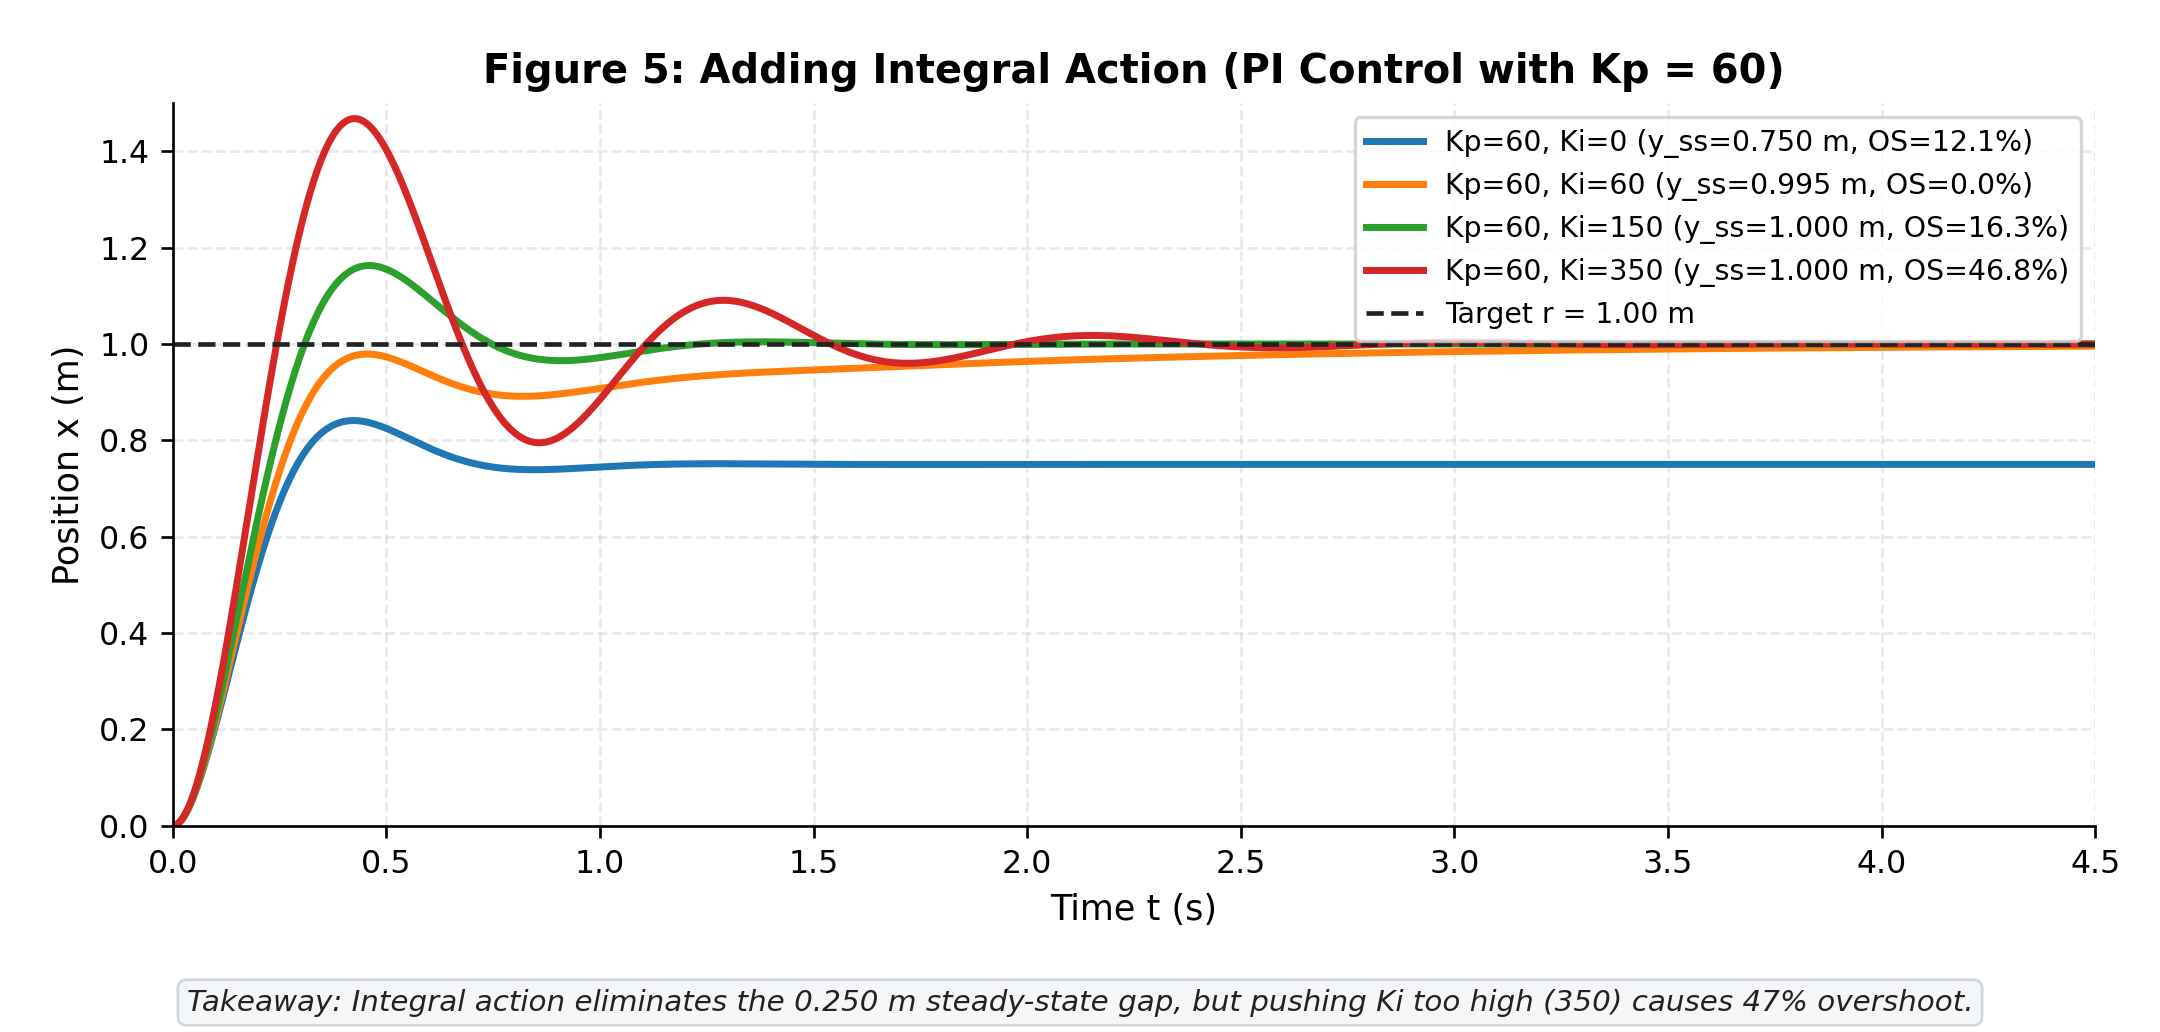
\includegraphics[width=0.90\textwidth]{figures/fig05_pi_control.png}
  \caption{PI control ($K_p = 60$): $K_i$ closes the $0.250\text{ m}$ gap completely, while excessive $K_i = 350$ causes $46.8\%$ overshoot.}
  \label{fig:pi}
\end{figure}

\subsection{Adding Derivative (PD): Braking the Bounce}
With $u = K_p(r - x) + K_d \frac{d}{dt}(r - x)$ and a constant target ($\dot{r} = 0$), $\dot{e} = -\dot{x}$, so Eq.~\eqref{eq:plant} becomes:
\begin{equation}
  \ddot{x} + \underbrace{(10 + K_d)}_{c_{\text{eff}}}\dot{x} + (20 + K_p)x = K_p r.
  \label{eq:pd_closed}
\end{equation}
\textbf{Exact damping calculation:} Comparing Eq.~\eqref{eq:pd_closed} with standard second-order form $\ddot{x} + 2\zeta\omega_n \dot{x} + \omega_n^2 x = \dots$, the derivative gain adds directly to physical damping ($c_{\text{eff}} = 10 + K_d$). For $K_p = 200$, $\omega_n = \sqrt{20 + 200} = \sqrt{220} = 14.832\text{ rad/s}$, so:
\begin{equation}
  \zeta = \frac{10 + K_d}{2\sqrt{220}}, \qquad
  \%\text{OS}_{\text{theory}} = \exp\!\left(-\frac{\pi \zeta}{\sqrt{1 - \zeta^2}}\right)\times 100\% \quad (\zeta < 1).
  \label{eq:zeta_os}
\end{equation}
Table~\ref{tab:pd} and Figure~\ref{fig:pd} verify Eq.~\eqref{eq:zeta_os}: increasing $K_d$ from $0$ to $15$ raises $\zeta$ from $0.337$ to $0.843$, slashing overshoot from $32.88\%$ to $0.69\%$ and cutting settling time from $0.749\text{ s}$ to $0.278\text{ s}$ (the tiny $0.4\%$ difference at $K_d=0$ comes from the $1\text{ ms}$ zero-order hold step).

\begin{table}[H]
  \centering
  \small
  \begin{tabular}{cccccc}
    \toprule
    $K_d$ ($\text{N}\cdot\text{s/m}$) & Effective $c_{\text{eff}}$ & Damping ratio $\zeta$ & Theory $\%\text{OS}$ & Simulated $\%\text{OS}$ & Settling $t_s$ ($\text{s}$) \\
    \midrule
    0  & 10 & 0.3371 & 32.47\% & 32.88\% & 0.749 \\
    5  & 15 & 0.5056 & 15.86\% & 16.03\% & 0.541 \\
    15 & 25 & 0.8427 & 0.73\%  & 0.69\%  & 0.278 \\
    25 & 35 & 1.1798 & 0.00\%  & 0.00\%  & 0.522 \\
    \bottomrule
  \end{tabular}
  \caption{PD control ($K_p = 200$): derivative action increases $\zeta$ and suppresses bouncing exactly as Eq.~\eqref{eq:zeta_os} predicts.}
  \label{tab:pd}
\end{table}

\begin{figure}[H]
  \centering
  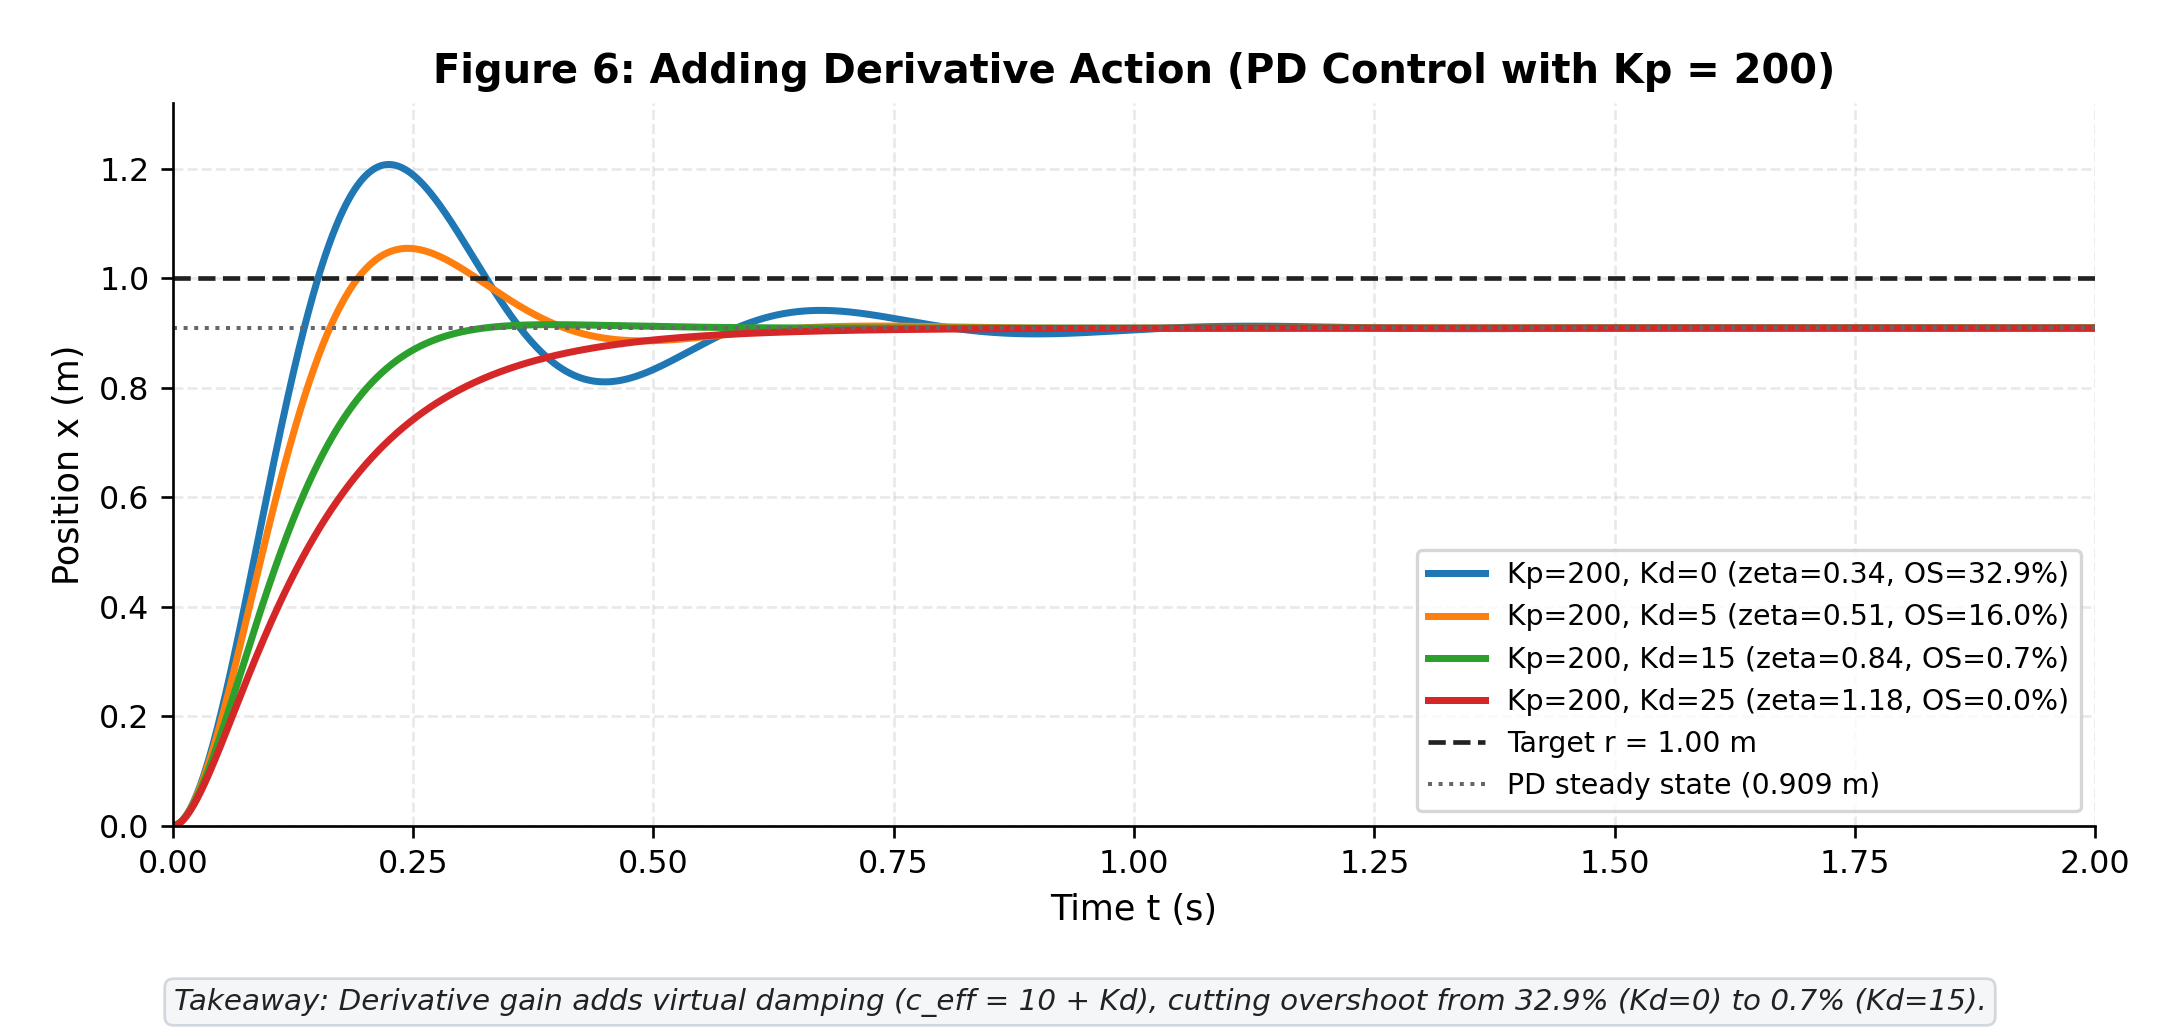
\includegraphics[width=0.90\textwidth]{figures/fig06_pd_control.png}
  \caption{PD control ($K_p = 200$): raising $K_d$ damps oscillations from $32.9\%$ overshoot down to $0.0\%$.}
  \label{fig:pd}
\end{figure}

% ============================================================================
\section{All Together: P vs.\ PI vs.\ PD vs.\ Full PID}
% ============================================================================
Keeping $K_p = 100$ fixed so the comparison is fair, Figure~\ref{fig:compare} and Table~\ref{tab:compare} compare P, PI, PD, and full PID on the same $0 \to 1\text{ m}$ task:
\begin{itemize}
  \item \textbf{P} ($100, 0, 0$) rises fast ($0.142\text{ s}$) but bounces ($20.16\%$ OS) and stops $0.167\text{ m}$ short.
  \item \textbf{PI} ($100, 120, 0$) eliminates the gap ($0.007\text{ m}$ at $2.5\text{ s}$, $0\text{ m}$ asymptotically) but oscillates ($14.57\%$ OS, slow $1.325\text{ s}$ settling).
  \item \textbf{PD} ($100, 0, 8$) tames overshoot to $1.06\%$ and settles in $0.359\text{ s}$, yet still stops $0.167\text{ m}$ short.
  \item \textbf{PID} ($100, 120, 8$) combines every strength: fast rise ($0.261\text{ s}$), under $1\%$ overshoot ($0.86\%$), rapid settling ($0.408\text{ s}$), and virtually zero error ($0.0001\text{ m}$).
\end{itemize}

\textbf{Final gain choice:} For the unconstrained test system, we choose \textbf{$K_p = 100\text{ N/m}$, $K_i = 120\text{ N/(m}\cdot\text{s)}$, $K_d = 8\text{ N}\cdot\text{s/m}$} because it achieves sub-1\% overshoot ($0.86\%$) and settles in $0.408\text{ s}$ without excessive peak force ($100.1\text{ N}$). (When the motor is capped at $\pm 30\text{ N}$ in Sections~7 and 9, we also test a more aggressive tuning $(120, 240, 12)$ to demonstrate how anti-windup rescues strong integral gains.)

\begin{table}[H]
  \centering
  \small
  \begin{tabular}{lccccc}
    \toprule
    Controller $(K_p, K_i, K_d)$ & Rise time $t_r$ ($\text{s}$) & Overshoot ($\%$) & Settling $t_s$ ($\text{s}$) & Steady error $e_{\text{ss}}$ ($\text{m}$) & Peak force ($\text{N}$) \\
    \midrule
    P   $(100, 0, 0)$   & 0.142 & 20.16\% & 0.761 & 0.1667 & 100.0 \\
    PI  $(100, 120, 0)$ & 0.157 & 14.57\% & 1.325 & 0.0067 & 100.9 \\
    PD  $(100, 0, 8)$   & 0.232 & 1.06\%  & 0.359 & 0.1667 & 100.0 \\
    \textbf{PID $(100, 120, 8)$} & \textbf{0.261} & \textbf{0.86\%} & \textbf{0.408} & \textbf{0.0001} & \textbf{100.1} \\
    \bottomrule
  \end{tabular}
  \caption{Step-response comparison of P, PI, PD, and full PID on the 1\,kg mass-spring-damper ($t_{\text{end}} = 2.5\text{ s}$).}
  \label{tab:compare}
\end{table}

\begin{figure}[H]
  \centering
  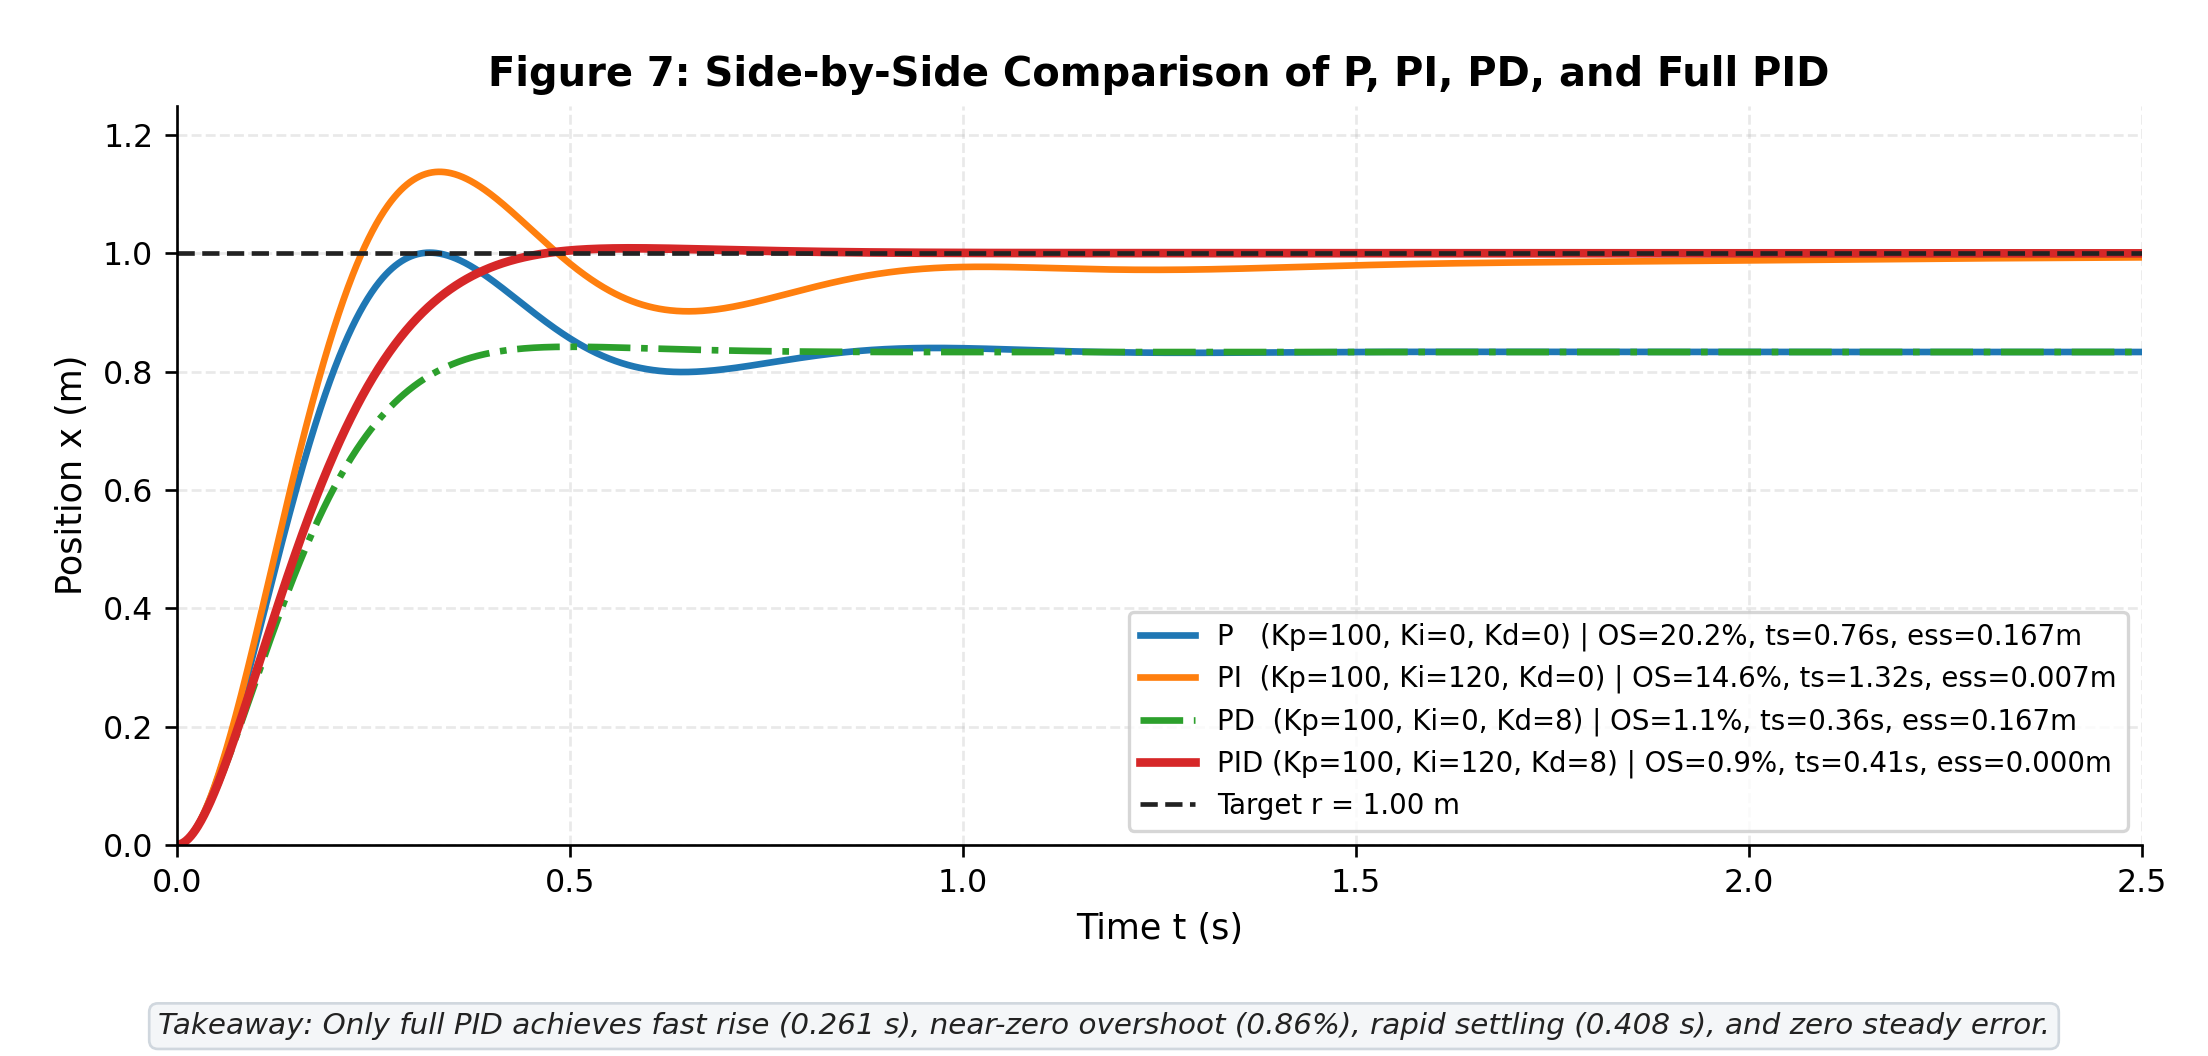
\includegraphics[width=0.90\textwidth]{figures/fig07_p_pi_pd_pid.png}
  \caption{P, PI, PD, and full PID compared directly: only PID hits $1.00\text{ m}$ fast without bouncing.}
  \label{fig:compare}
\end{figure}

% ============================================================================
\section{Real-World Problems (and How to Fix Them)}
% ============================================================================
Ideal math ignores motor limits, noisy sensors, instant target jumps, and finite computer speed. Here are the four classic pitfalls on our test system (using PID $(120, 240, 12)$) and the exact engineering fix for each.

\subsection*{(a) Actuator Limit ($\pm 30\text{ N}$) and Integrator Windup}
\textbf{Problem:} Real motors saturate. If the motor can push at most $30\text{ N}$, the block takes longer to reach $1\text{ m}$. Meanwhile, a naive integrator keeps summing error and ``winds up'' to $68.6\text{ N}$---more than double the motor limit. Even after the block passes $1.0\text{ m}$, the huge stored $I$ term keeps pinning the motor at $+30\text{ N}$, causing \textbf{26.9\% overshoot} and $2.05\text{ s}$ settling.

\textbf{Fix (Conditional Integration / Anti-Windup):} Stop adding to the integral whenever the output is already saturated and the error pushes further into saturation. Result (Figure~\ref{fig:windup}): overshoot drops from \textbf{26.9\% to 0.0\%} and settling time improves from \textbf{2.05\,s to 0.83\,s}.

\begin{figure}[H]
  \centering
  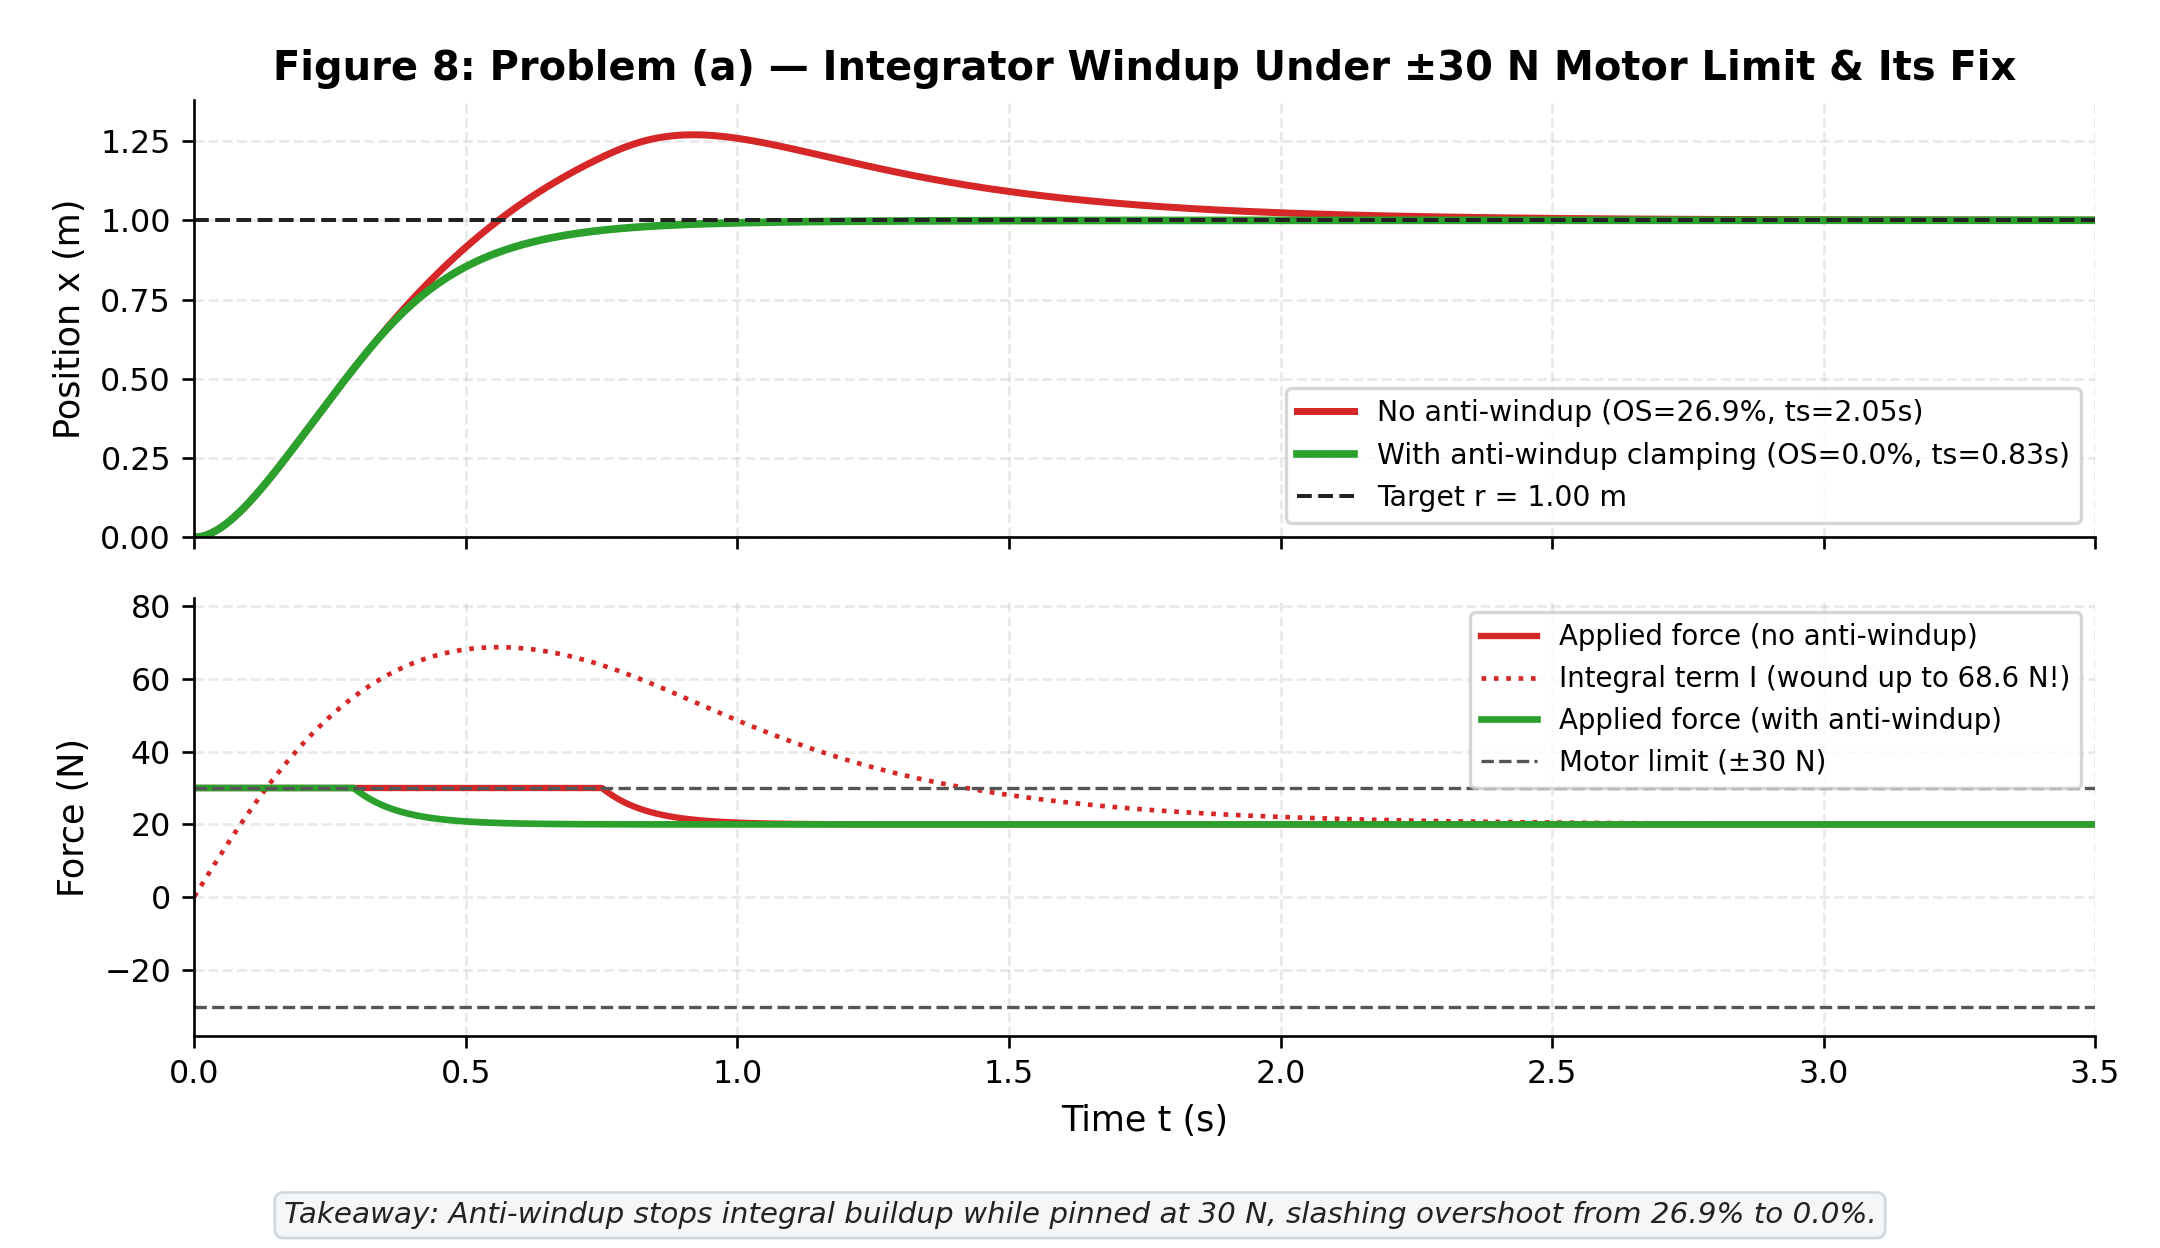
\includegraphics[width=0.90\textwidth]{figures/fig08_windup.png}
  \caption{Integrator windup under a $\pm 30\text{ N}$ limit vs.\ conditional-integration anti-windup.}
  \label{fig:windup}
\end{figure}

\subsection*{(b) Noisy Sensor ($\pm 1\text{ mm}$) and Jumpy Derivative}
\textbf{Problem:} Suppose an encoder has $\pm 1\text{ mm}$ ($0.001\text{ m}$) measurement noise at $1\text{ kHz}$ ($\Delta t = 0.001\text{ s}$). Dividing a $1\text{ mm}$ jump by $0.001\text{ s}$ produces $\pm 1\text{ m/s}$ fake velocity spikes, which $K_d = 12$ amplifies into \textbf{39.7\,N peak-to-peak} motor chatter ($\sigma = 6.86\text{ N}$) even while sitting still!

\textbf{Fix (Low-Pass Derivative Filter):} Smooth the derivative using a first-order low-pass filter with time constant $\tau_d = 0.025\text{ s}$:
$D_k = \frac{\tau_d D_{k-1} + \Delta t \, d_k}{\tau_d + \Delta t}$. Result (Figure~\ref{fig:noise}): steady-state motor chatter drops by \textbf{96.8\%}, from $39.7\text{ N}$ down to \textbf{1.26\,N} peak-to-peak ($\sigma = 0.24\text{ N}$).

\begin{figure}[H]
  \centering
  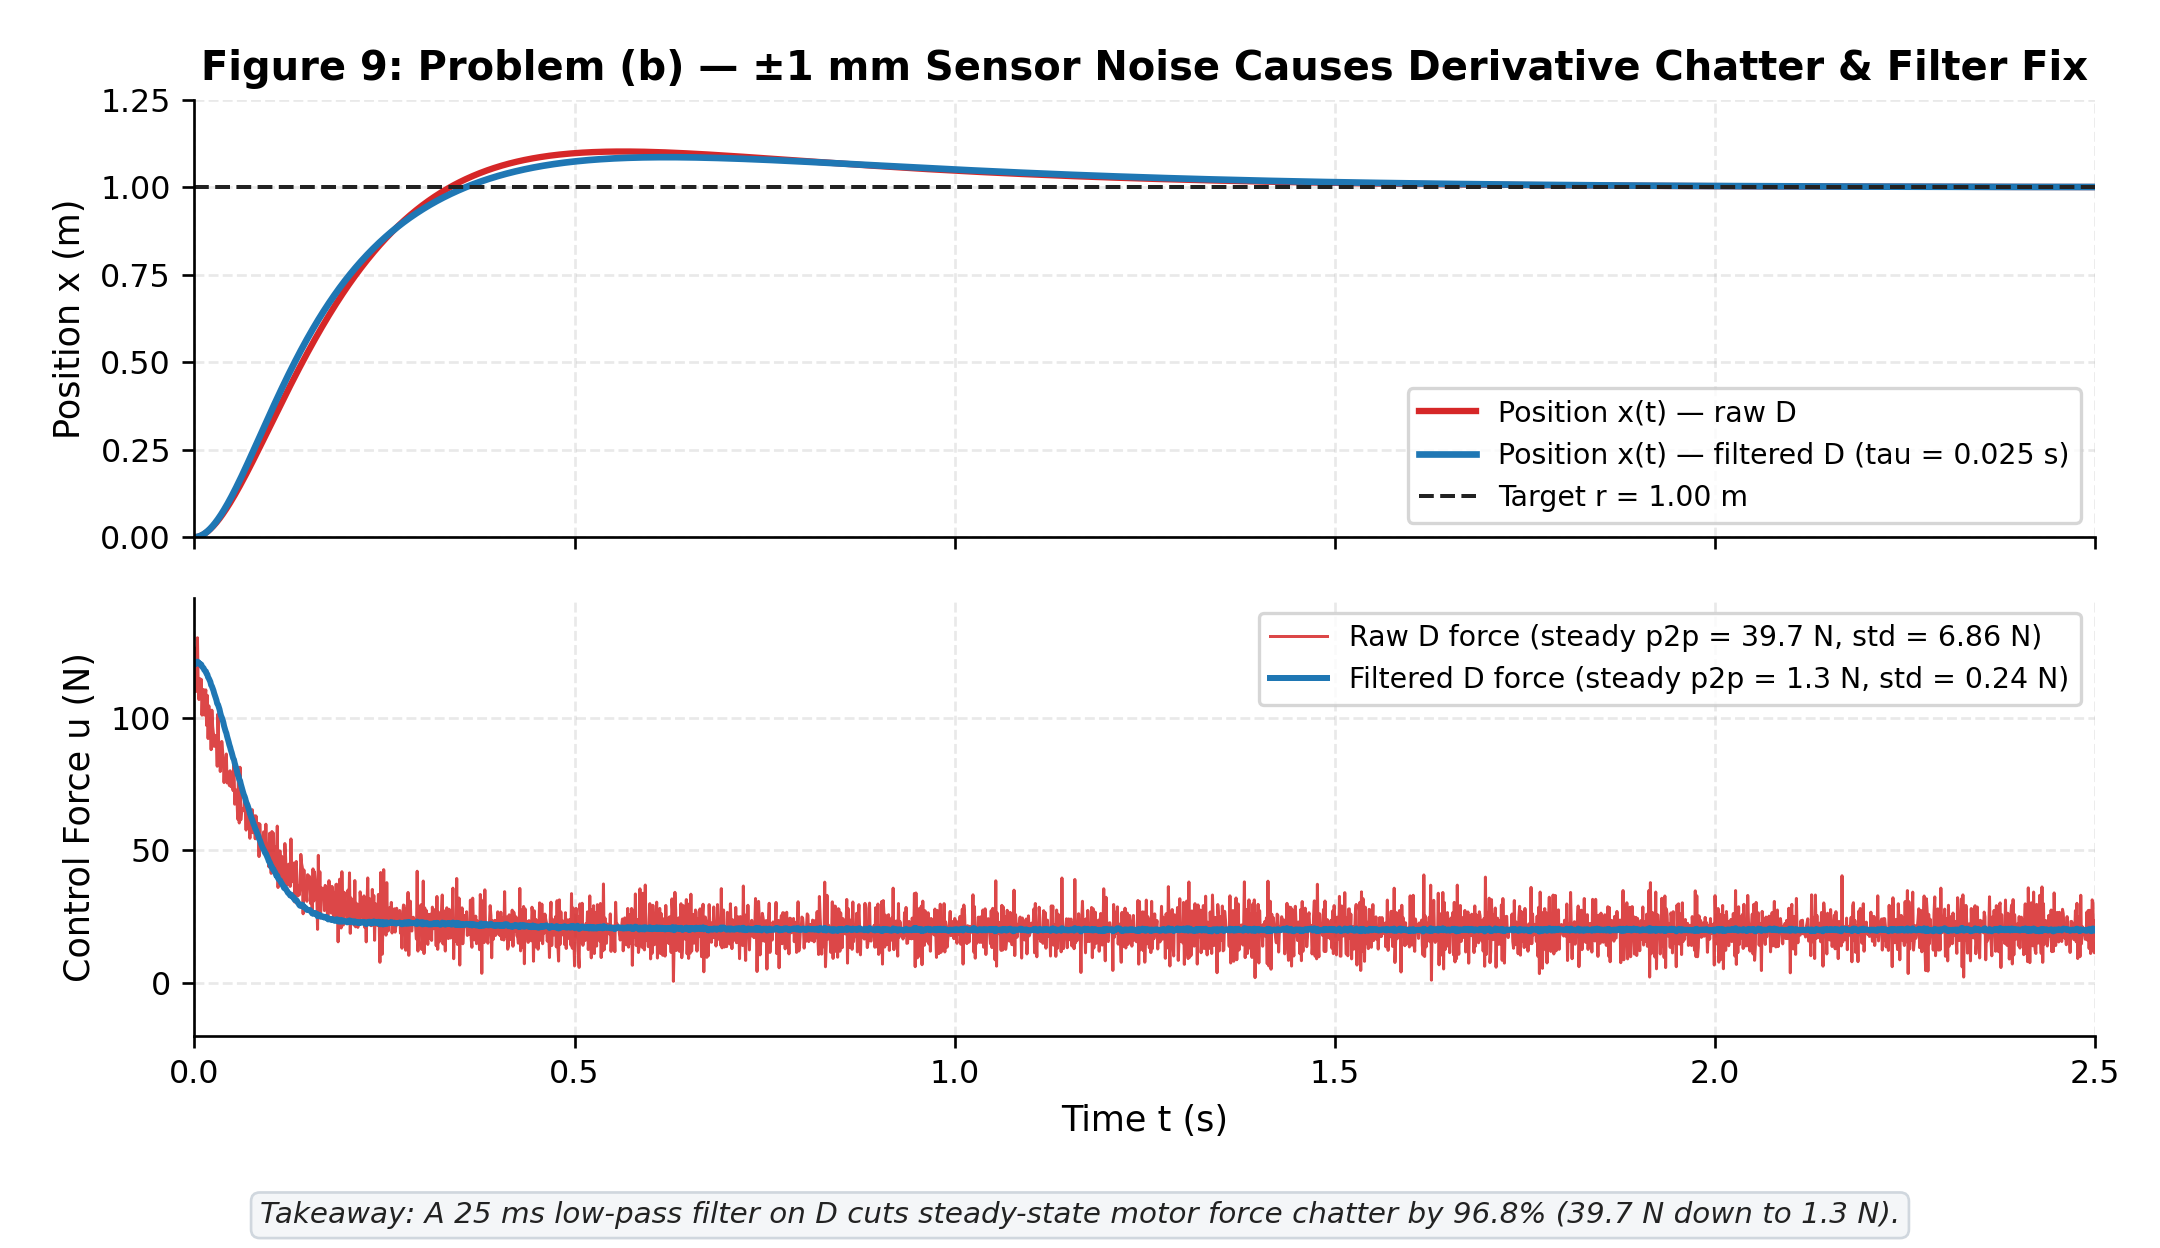
\includegraphics[width=0.90\textwidth]{figures/fig09_noise.png}
  \caption{Raw derivative turns $\pm 1\text{ mm}$ sensor noise into $39.7\text{ N}$ force chatter; a $25\text{ ms}$ filter cuts it by $96.8\%$.}
  \label{fig:noise}
\end{figure}

\subsection*{(c) Sudden Target Step and Derivative Kick}
\textbf{Problem:} When the setpoint jumps instantly from $0$ to $1\text{ m}$ at $t = 0.5\text{ s}$ (with $\Delta t = 0.001\text{ s}$), $\frac{e_k - e_{k-1}}{\Delta t}$ becomes $\frac{1.0}{0.001} = 1000\text{ m/s}$, firing a massive \textbf{12,120\,N spike} (over $100\times$ normal force) that can trip breakers or strip gears.

\textbf{Fix (Derivative on Measurement):} Since $\frac{de}{dt} = \frac{dr}{dt} - \frac{dy}{dt}$ and the physical block cannot teleport, compute $D$ purely from $-\frac{y_k - y_{k-1}}{\Delta t}$. Result (Figure~\ref{fig:kick}): the $12{,}120\text{ N}$ spike vanishes completely, capping peak force at \textbf{120.2\,N}.

\begin{figure}[H]
  \centering
  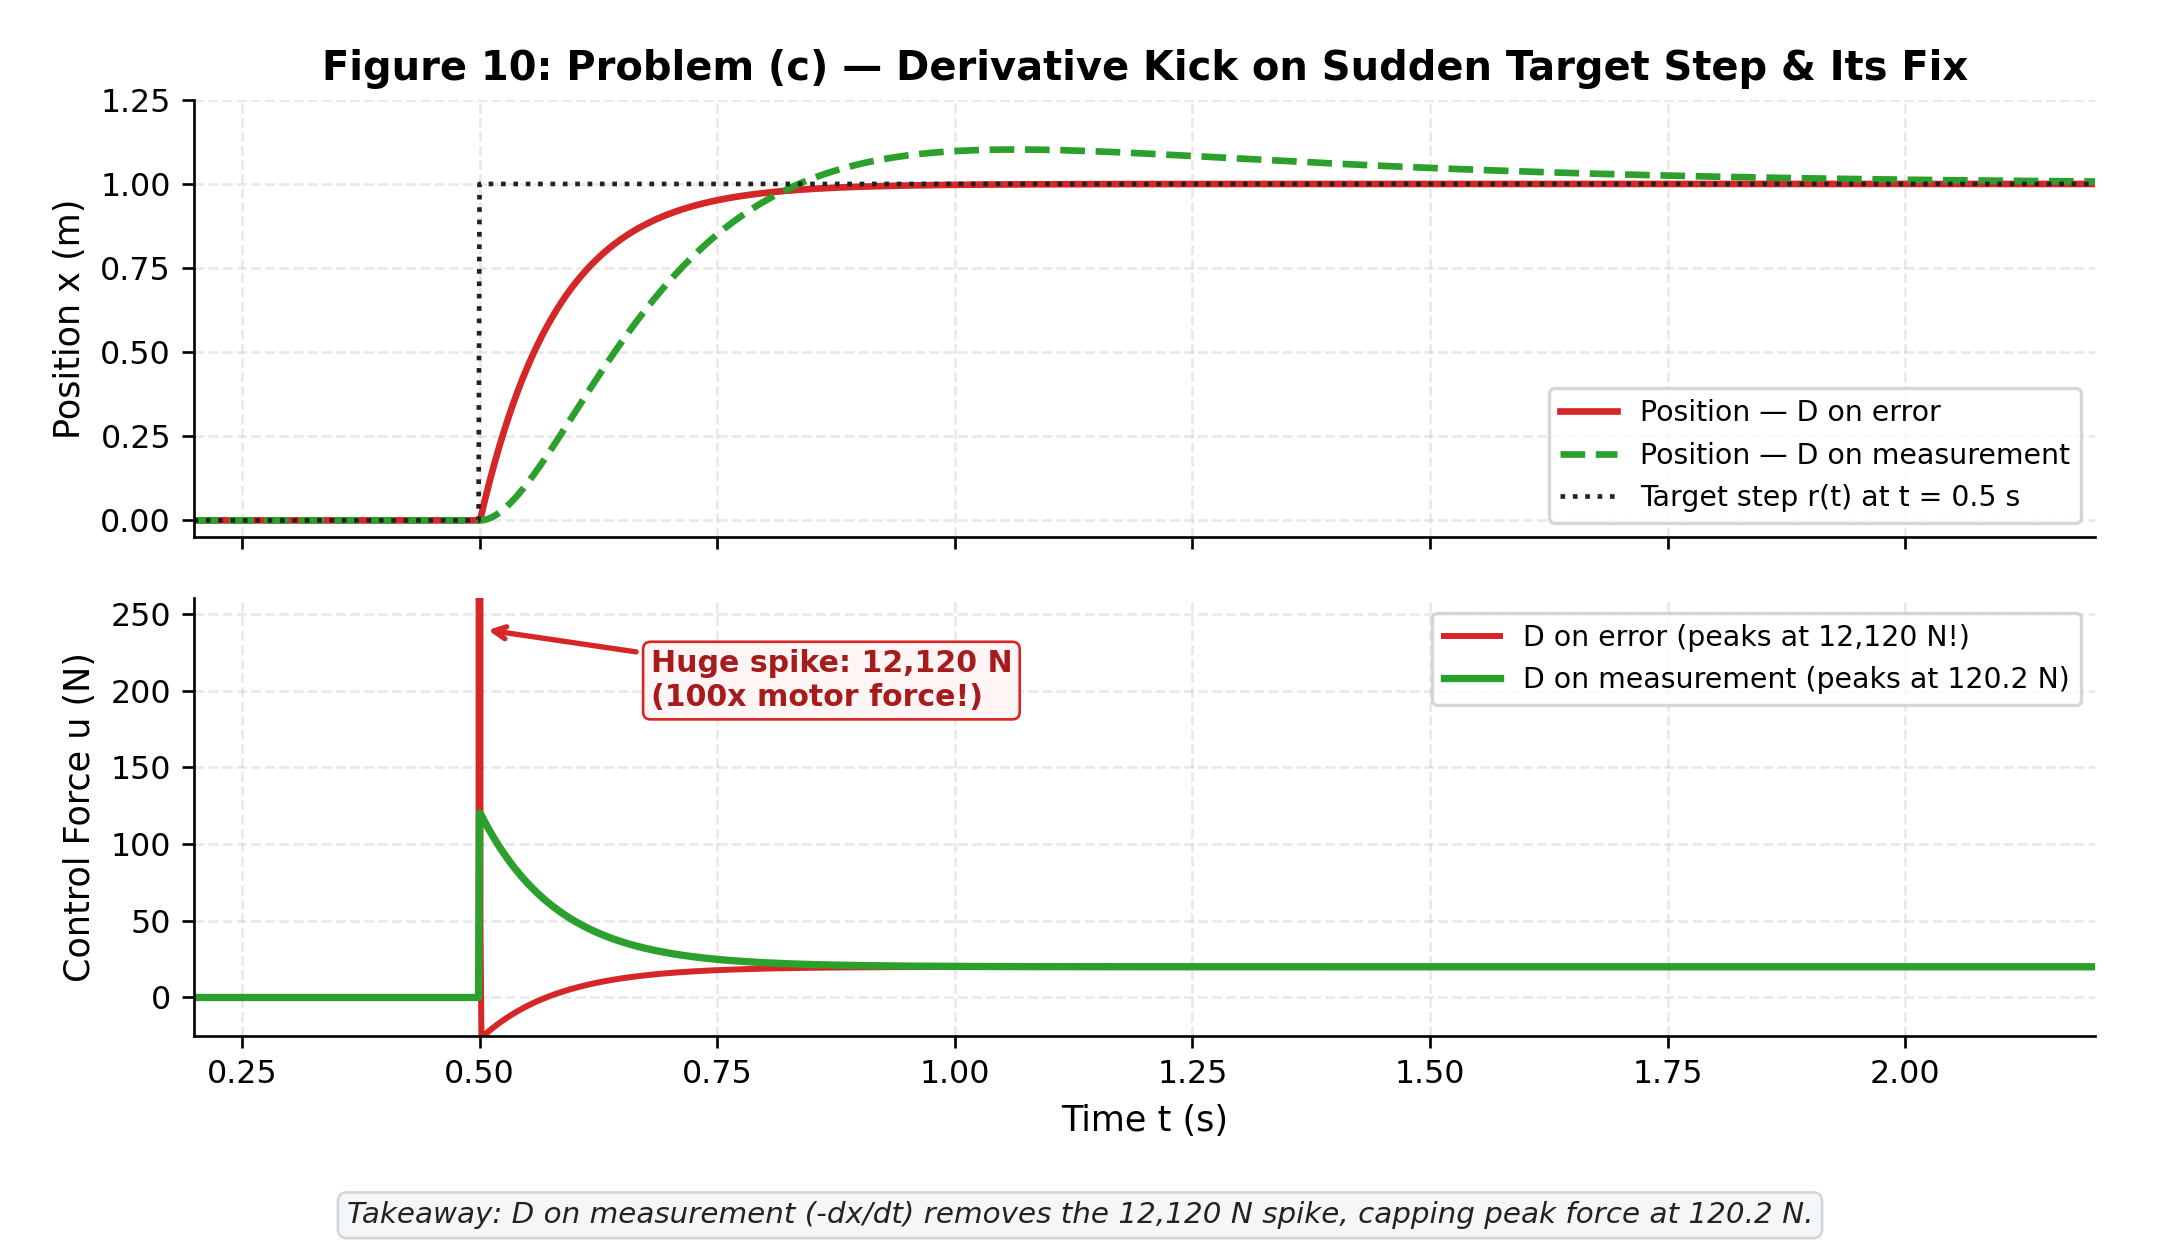
\includegraphics[width=0.90\textwidth]{figures/fig10_derivative_kick.png}
  \caption{Derivative-on-measurement eliminates the $12{,}120\text{ N}$ setpoint kick.}
  \label{fig:kick}
\end{figure}

\subsection*{(d) Slow Computer Update Rate ($\Delta t$ Too Large)}
\textbf{Problem:} Holding an outdated force command between slow updates injects an average delay of $\Delta t/2$, eroding phase margin. On our system (rise time $\approx 0.23\text{ s}$), Figure~\ref{fig:dt} shows that $\Delta t = 0.001\text{ s}$ ($1000\text{ Hz}$) and $\Delta t = 0.060\text{ s}$ ($17\text{ Hz}$) behave smoothly ($10.2\%$ and $8.4\%$ overshoot), $\Delta t = 0.100\text{ s}$ ($10\text{ Hz}$) nearly doubles overshoot to \textbf{18.1\%} with visible ringing, and $\Delta t = 0.165\text{ s}$ ($6\text{ Hz}$) goes \textbf{unstable} (oscillating wildly up to $1.76\text{ m}$). \textbf{Rule of thumb:} sample at least $10\times$ faster than the closed-loop rise time ($\Delta t \le t_r / 10$, i.e.\ $\ge 50\text{--}200\text{ Hz}$ here).

\begin{figure}[H]
  \centering
  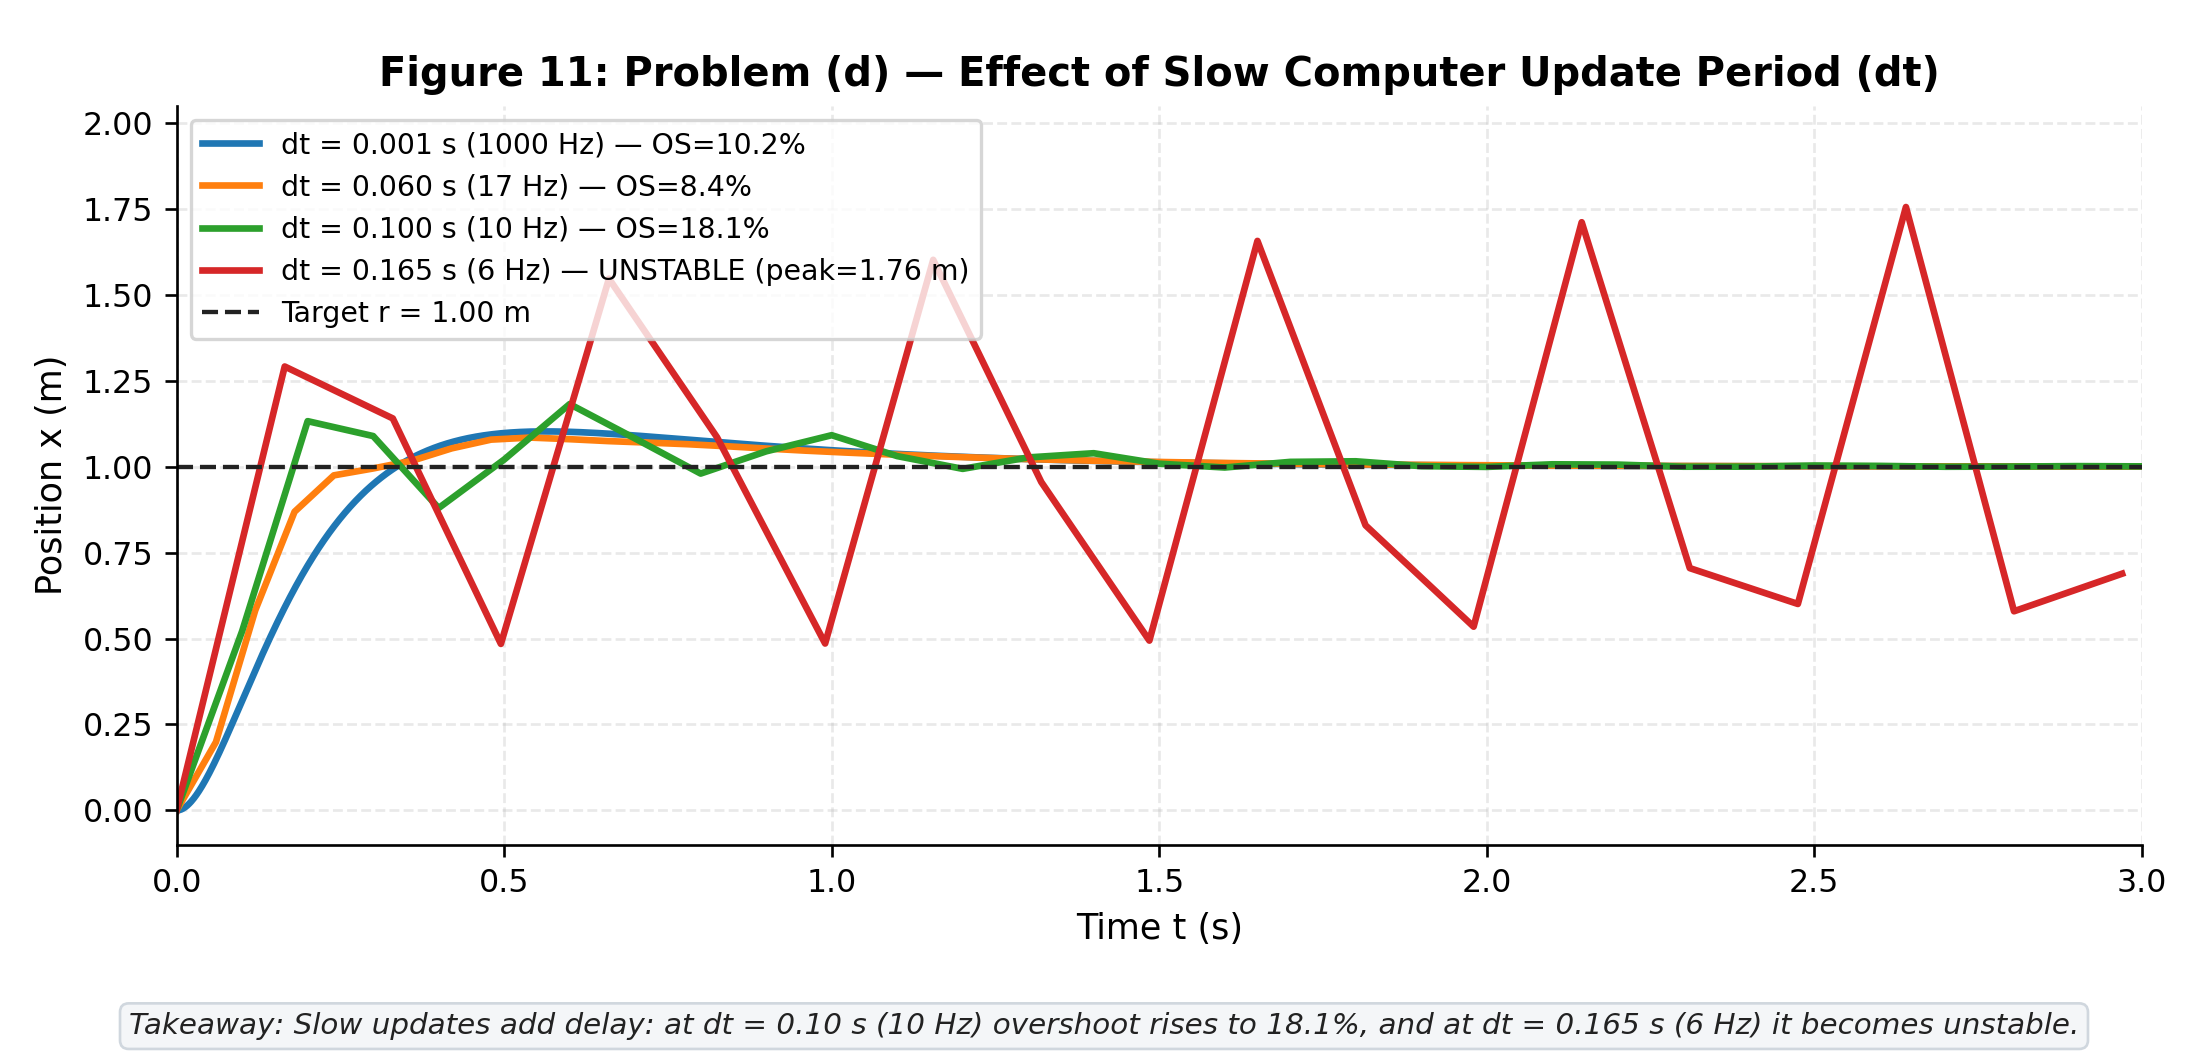
\includegraphics[width=0.90\textwidth]{figures/fig11_sample_rate.png}
  \caption{Increasing the sample period $\Delta t$ adds phase lag, turning a clean response into unstable oscillations at $6\text{ Hz}$.}
  \label{fig:dt}
\end{figure}

% ============================================================================
\section{Choosing the Gains (Manual \& Ziegler--Nichols)}
% ============================================================================
\textbf{Step-by-step manual tuning recipe:}
\begin{enumerate}
  \item Set $K_i = 0$ and $K_d = 0$. Raise $K_p$ until the system moves briskly toward the target with moderate bounce (around $10\text{--}25\%$ overshoot).
  \item Raise $K_d$ (with a derivative filter $\tau_d$ if noisy) until the overshoot and bouncing disappear.
  \item Raise $K_i$ slowly until any steady-state offset vanishes within your desired settling time.
  \item Fine-tune: if adding $K_i$ brings back overshoot, nudge $K_d$ up slightly or trim $K_p$ by $10\text{--}20\%$.
\end{enumerate}

\textbf{Ziegler--Nichols (ZN) ultimate-gain test on a second system, $G(s) = \frac{1}{(s+1)^3}$:}
In time domain, this third-order plant obeys $\dddot{y} + 3\ddot{y} + 3\dot{y} + y = u$. Using P-only control, we raise $K_p$ until the output swings steadily without growing or decaying (Figure~\ref{fig:zn}, left). Analytically, the phase of $G(j\omega) = (1+j\omega)^{-3}$ hits $-180^\circ$ when $3\arctan(\omega_u) = 180^\circ \Rightarrow \omega_u = \sqrt{3}\text{ rad/s}$, where $|G(j\omega_u)| = 2^{-3} = \tfrac{1}{8}$. Thus the exact ultimate gain and period are:
\[
  K_u = 8.0, \qquad T_u = \frac{2\pi}{\omega_u} = \frac{2\pi}{\sqrt{3}} = 3.628\text{ s} \quad (\text{simulation measures } T_u = 3.630\text{ s}).
\]
Applying the classic ZN recipe (Table~\ref{tab:zn}) gives PID gains $(K_p, K_i, K_d) = (4.80, 2.646, 2.177)$. As Figure~\ref{fig:zn} (right) shows, ZN reacts fast ($t_r = 0.949\text{ s}$) because it targets ``quarter-wave decay,'' but suffers \textbf{52.4\% overshoot} and takes \textbf{9.98\,s} to settle. Trimming aggression to \textbf{$(K_p, K_i, K_d) = (3.40, 0.70, 2.60)$} cuts overshoot from \textbf{52.4\% to 1.25\%} and speeds settling from \textbf{9.98\,s to 2.69\,s} ($3.7\times$ faster!).

\begin{table}[H]
  \centering
  \small
  \begin{tabular}{lccccc}
    \toprule
    Tuning Rule & $K_p$ & $K_i$ & $K_d$ & Applied Values on $1/(s+1)^3$ & Result ($t_r$, $\%\text{OS}$, $t_s$) \\
    \midrule
    ZN P   & $0.50\,K_u$ & $0$ & $0$ & $(4.00, 0, 0)$ & $e_{\text{ss}} = 0.20$ \\
    ZN PI  & $0.45\,K_u$ & $0.54\,K_u / T_u$ & $0$ & $(3.60, 1.191, 0)$ & oscillatory \\
    ZN PID & $0.60\,K_u$ & $1.20\,K_u / T_u$ & $0.075\,K_u T_u$ & $(4.800, 2.646, 2.177)$ & $0.949\text{ s},\ 52.41\%,\ 9.980\text{ s}$ \\
    \textbf{Improved PID} & \multicolumn{3}{c}{Reduced $K_p, K_i$; higher $K_d$} & \textbf{(3.400, 0.700, 2.600)} & \textbf{1.629\,s, 1.25\%, 2.690\,s} \\
    \bottomrule
  \end{tabular}
  \caption{Ziegler--Nichols recipe table and performance improvement on $G(s) = 1/(s+1)^3$.}
  \label{tab:zn}
\end{table}

\begin{figure}[H]
  \centering
  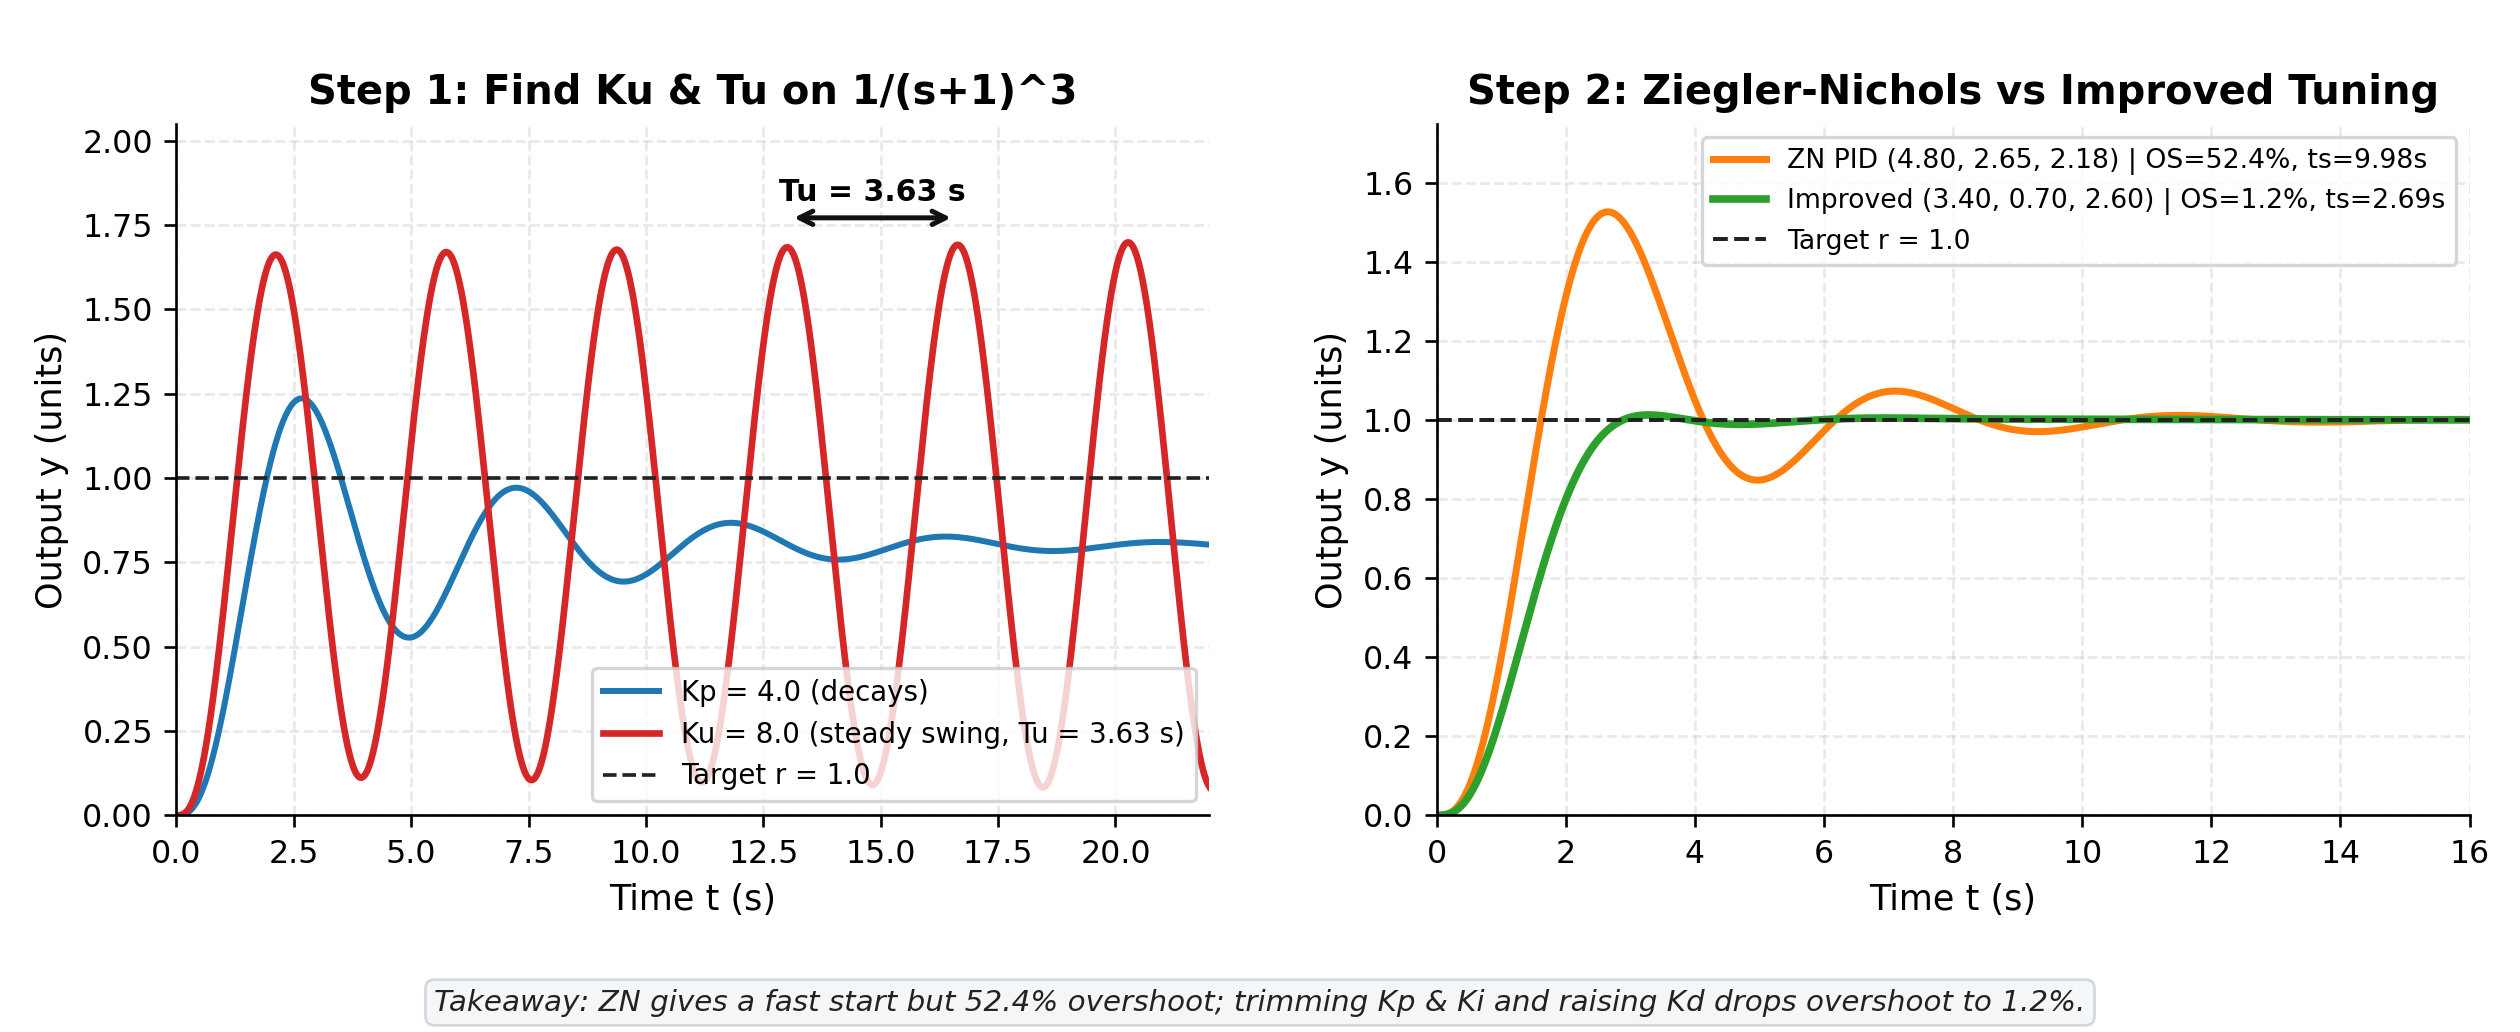
\includegraphics[width=0.98\textwidth]{figures/fig12_ziegler_nichols.png}
  \caption{Left: Finding $K_u = 8.0$ and $T_u = 3.63\text{ s}$ on $1/(s+1)^3$. Right: ZN PID ($52.4\%$ OS) vs.\ improved PID ($1.25\%$ OS).}
  \label{fig:zn}
\end{figure}

% ============================================================================
\newpage
\section{The Code: Reusable PID with All Real-World Fixes}
% ============================================================================
Below is the core \texttt{update()} logic from \texttt{pid\_controller.py}, combining output clamping, conditional-integration anti-windup, derivative-on-measurement, and the first-order derivative filter:

\begin{Verbatim}[fontsize=\footnotesize, frame=single, framesep=4pt]
class PIDController:
    def __init__(self, kp, ki, kd, u_min=-float("inf"), u_max=float("inf"),
                 anti_windup=True, derivative_on_measurement=True, d_filter_tau=0.0):
        self.kp, self.ki, self.kd = float(kp), float(ki), float(kd)
        self.u_min, self.u_max = float(u_min), float(u_max)
        self.anti_windup = anti_windup
        self.derivative_on_measurement = derivative_on_measurement
        self.d_filter_tau = float(d_filter_tau)
        self.reset()

    def update(self, setpoint, measurement, dt):
        error = setpoint - measurement
        p_term = self.kp * error

        # Derivative on measurement avoids setpoint kick
        if self.derivative_on_measurement:
            raw_d = 0.0 if self.prev_measurement is None else -(measurement - self.prev_measurement) / dt
        else:
            raw_d = 0.0 if self.prev_error is None else (error - self.prev_error) / dt

        # Low-pass filter on D suppresses high-frequency sensor noise
        if self.d_filter_tau > 0.0:
            alpha = dt / (self.d_filter_tau + dt)
            self.d_filtered = (1.0 - alpha) * self.d_filtered + alpha * raw_d
        else:
            self.d_filtered = raw_d
        d_term = self.kd * self.d_filtered

        # Conditional integration anti-windup
        cand_i = self.integral + error * dt
        u_cand = p_term + self.ki * cand_i + d_term
        if not (self.anti_windup and ((u_cand > self.u_max and error > 0) or
                                      (u_cand < self.u_min and error < 0))):
            self.integral = cand_i

        u = max(self.u_min, min(self.u_max, p_term + self.ki * self.integral + d_term))
        self.prev_error, self.prev_measurement = error, measurement
        return u
\end{Verbatim}

Running \texttt{python3 run\_section9\_demo.py} on our $1\text{ kg}$ test plant at $200\text{ Hz}$ ($\Delta t = 0.005\text{ s}$) with $\pm 30\text{ N}$ motor limit, $\pm 1\text{ mm}$ sensor noise, and a sudden step at $t = 0.3\text{ s}$ produces the exact terminal output below and Figure~\ref{fig:sec9}:
\begin{Verbatim}[fontsize=\footnotesize, frame=single, framesep=4pt]
=== Reusable PIDController Run (Test System) ===
Gains          : Kp=120.0, Ki=240.0, Kd=12.0
Limits / Filter: u in [-30.0, 30.0] N, tau_d=0.025 s
Rise time      : 0.483 s
Overshoot      : 0.17 %
Settling time  : 0.840 s
Steady error   : 0.0002 m
Peak force     : 30.00 N
Steady u ripple: 1.21 N (peak-to-peak)
\end{Verbatim}

\begin{figure}[H]
  \centering
  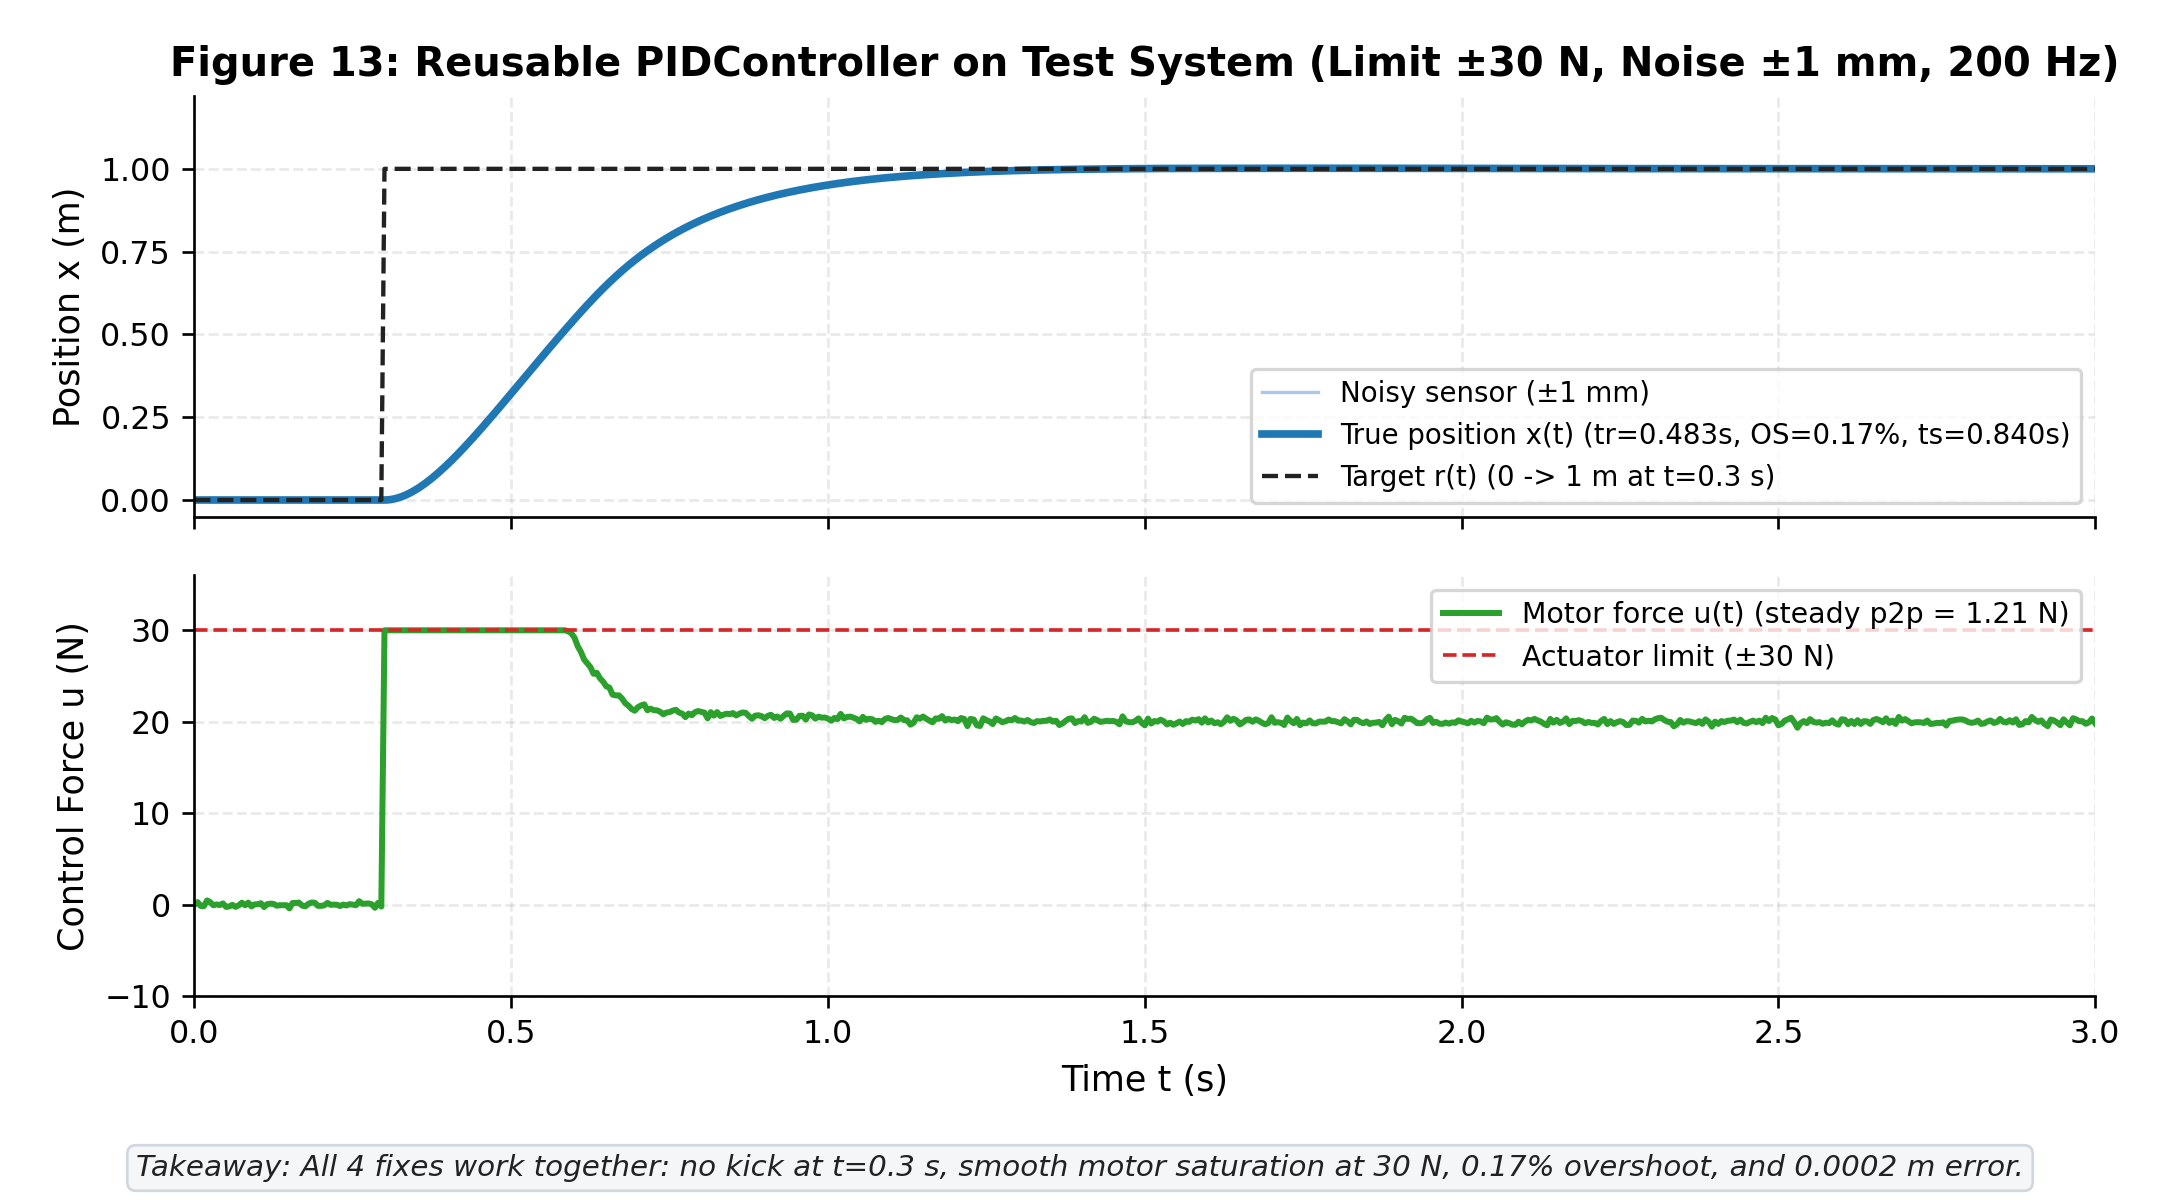
\includegraphics[width=0.88\textwidth]{figures/fig13_reusable_pid_demo.png}
  \caption{Production \texttt{PIDController} running with $\pm 30\text{ N}$ limit, $\pm 1\text{ mm}$ noise, and a step at $t = 0.3\text{ s}$.}
  \label{fig:sec9}
\end{figure}

% ============================================================================
\section{Real Robots \& Common Myths}
% ============================================================================

\subsection*{Five Real-World Examples of PID Control}
\begin{enumerate}
  \item \textbf{DC Motor Speed Control:} \textit{Setpoint:} target RPM (e.g.\ $1500\text{ RPM}$). \textit{Sensor:} optical encoder ticks/second. \textit{Actuator:} PWM voltage to motor driver. \textit{Roles:} P gives quick spin-up, I overcomes bearing friction and load torque so RPM hits target exactly, and D is often tiny or zero because speed loops are first-order and encoders are noisy.
  \item \textbf{Quadcopter Drone (Attitude \& Altitude):} \textit{Setpoint:} desired roll/pitch angle ($0^\circ$ hover) or height ($2\text{ m}$). \textit{Sensor:} IMU gyroscope/accelerometer ($500\text{--}1000\text{ Hz}$) and barometer/lidar. \textit{Actuator:} four brushless motor speeds. \textit{Roles:} P levels the drone, D damps fast angular flips from wind gusts, and I trims out battery voltage sag or off-center payload weight.
  \item \textbf{Robot Arm Joint Position:} \textit{Setpoint:} joint angle $\theta_{\text{target}}$. \textit{Sensor:} joint optical/magnetic encoder. \textit{Actuator:} servo torque. \textit{Roles:} P pulls the arm to angle, I holds the arm up against gravity (just like holding our $20\text{ N}$ spring!), and D prevents mechanical overshoot and ringing when stopping.
  \item \textbf{Differential-Drive Line Follower:} \textit{Setpoint:} line centered under array ($e = 0$). \textit{Sensor:} IR reflectance sensor array. \textit{Actuator:} left/right wheel speed difference $\Delta v$. \textit{Roles:} P steers back toward the tape, D reacts early to sharp S-curves so the robot does not fly off, and I is usually near zero so corners do not wind up steering.
  \item \textbf{Car Cruise Control:} \textit{Setpoint:} $100\text{ km/h}$. \textit{Sensor:} wheel-speed sensor. \textit{Actuator:} throttle opening. \textit{Roles:} P adds gas when slowing down, I holds extra throttle climbing a long hill so speed does not sag, and D smooths transitions without jerky acceleration.
\end{enumerate}

\newpage
\subsection*{Five Common Myths About PID---Corrected}
\begin{enumerate}
  \item \textbf{Myth: ``You always need all three P, I, and D.''} \\
  \textit{Reality:} Use only what the physics demands. Motor velocity and thermal loops frequently use \textbf{PI} (noise makes D counterproductive), while pure-integrator systems like some angle loops work well with \textbf{PD} (no I needed).
  \item \textbf{Myth: ``Higher $K_p$ always makes a system faster and more accurate.''} \\
  \textit{Reality:} Raising $K_p$ lowers steady-state error only up to a point; too much $K_p$ lowers damping ratio $\zeta$ (Eq.~\eqref{eq:zeta_os}), causing violent overshoot and eventual instability.
  \item \textbf{Myth: ``You must know exact physics equations to use PID.''} \\
  \textit{Reality:} PID is model-free in operation---methods like manual tuning and Ziegler--Nichols (Section~8) tune a black-box machine solely by watching how it responds.
  \item \textbf{Myth: ``Derivative D only amplifies noise and should never be used.''} \\
  \textit{Reality:} Unfiltered D amplifies noise ($39.7\text{ N}$ chatter in Figure~\ref{fig:noise}), but adding a simple low-pass filter ($\tau_d$) cuts chatter by $>96\%$ while keeping D's life-saving damping.
  \item \textbf{Myth: ``The integral term is harmless when the actuator hits max power.''} \\
  \textit{Reality:} Without anti-windup, the integral winds up blindly during saturation ($68.6\text{ N}$ in Figure~\ref{fig:windup}), causing severe overshoot ($26.9\%$) long after the target is reached.
\end{enumerate}

\subsection*{Interview Preparation: Predicting What Happens When Parameters Change}
In a technical evaluation or design review, you are frequently asked to predict the effect of physical parameter changes before re-running code. Table~\ref{tab:interview} provides the physical and mathematical rationale for each parameter shift:

\begin{table}[H]
  \centering
  \small
  \begin{tabular}{p{2.8cm} p{5.2cm} p{7.8cm}}
    \toprule
    \textbf{Parameter Change} & \textbf{Predicted System Response} & \textbf{Physical \& Mathematical Reason} \\
    \midrule
    Increase mass $m$ & Slower rise; higher overshoot; longer settling $t_s$ & Higher inertia; $\omega_n = \sqrt{k_{\text{tot}}/m}\downarrow$, $\zeta \propto 1/\sqrt{m}\downarrow$. \\
    Increase spring $k$ & Faster rise; larger steady error (if P-only) & Stiffer spring; higher natural frequency; requires larger $u_{\infty} = k\cdot r$. \\
    Increase damping $c$ & Slower rise; lower overshoot; faster settling & Adds physical damping force $-c\dot{x}$; raises damping ratio $\zeta$. \\
    Increase gain $K_p$ & Faster rise; smaller $e_{\text{ss}}$; higher overshoot & Virtual spring stiffens; $\omega_n\uparrow$, but $\zeta \propto 1/\sqrt{k+K_p}\downarrow$. \\
    Increase gain $K_i$ & Faster $e_{\text{ss}}\to 0$; increased overshoot & Erases lingering gap; adds phase lag; risks windup if saturated. \\
    Increase gain $K_d$ & Dramatically cuts overshoot; dampens bounce & Adds virtual damping $c_{\text{eff}} = c + K_d$; raises $\zeta$; sensitive to noise. \\
    Lower limit $u_{\max}$ & Slower initial rise; severe windup if naive & Actuator saturates longer; anti-windup clamping is mandatory. \\
    Increase noise $\sigma$ & Motor chattering and force ripple spike & D-term takes derivative of high-frequency noise; requires filter $\tau_d$. \\
    Increase step $\Delta t$ & Increased overshoot; ringing; instability & Zero-order hold injects $\Delta t/2$ delay; erodes phase margin. \\
    \bottomrule
  \end{tabular}
  \caption{Quick prediction matrix: how physical and controller parameters alter closed-loop performance.}
  \label{tab:interview}
\end{table}

\begin{notebox}[Note on AI Tools]
AI coding assistance was used to help draft and refine LaTeX layout, structure beginner-friendly analogies, and cross-check Python plotting code. All equations, analytical derivations (steady-state error, damping ratio $\zeta$, ultimate gain $K_u = 8$, period $T_u = 2\pi/\sqrt{3}$), and simulation metrics were independently verified against pure-NumPy code runs.
\end{notebox}

\end{document}
